

\chapter{ 线性规划问题 (1) }

%正文区
\section{回顾}
到现在为止,我们可以整理一下这门课到底讲什么。回顾一下已经学过的内容,理清思路。

我们把一个问题建模成组合优化的问题后,首先想到的是能否正面攻击它。第一个观察是,这个问题是否可以分成独立的子问题呢?如果是,基本的思路是规约(Reduction),如使用divide and Conquer 算法。 如果还有最优子结构的性质,可用动态规划(dynamic programming)算法。如果进一步还有贪心选择的性质,可用贪心(Greedy)算法。当然也可以在观察到问题可以分解时,直接应用贪心算法。上节课讲过,可以用部分解的枚举树,直接做贪心算法。以上这些是我们已经学习过的内容,通过对一个问题怎样观察,观察到怎样的性质,来决定我们使用什么算法。

今天所学的内容是我们思路的一个转折点,如果我们观察到一个问题不能够分解,或者我们不愿意进行分解,这个时候怎么办呢?那就只有一种办法,逐步改进法(Improvement)。这里面包括线性规划算法(Linear programming algorithm),网络流算法(Network flow algorithm),局部搜索算法(Local Search Algorithms) 中的蒙特·卡罗方法( Monte Carlo method)LS/MC,分支限界方法(branch and bound method),等等。

\section{本章内容}

我们先从实际问题讲起,然后讲这些实际问题的数学建模。这些问题包括:饮食问题,最大流问题, 最小费用流,多物品流,SAT问题。接着我们考虑怎样把这些问题建模成数学的线性规划的问题,以及对于线性规划的直观认识和求解方法,包括单纯型算法,内联法,椭球法。

最后,我们介绍领域内一个新的重要的方法,平滑复杂度算法。它完美的回答了,为什么单纯型算法本身具有指数级复杂度,却往往在实际应用中可以做到在线性复杂度的时间内解决问题。

\section{几个例子}
\subsection{第一个例子:饮食问题}
\textbf{问题:}
%图片
\newpage
\begin{table}
\begin{center}
  { \begin{tabular}{l|ccc|c}\hline
       Food & Energy & Protein & Calcium  & Price \\
 \hline
 Oatmeal & 110 & 4 & 2 & 3 \\
 Whole milk & 160 & 8 & 285 & 9 \\
 Cherry pie & 420 & 4 & 22 & 20 \\
 Pork with beans & 260 & 14 & 80 & 19 \\
\hline
\end{tabular}} {}%
\end{center}

\end{table}


大家考虑这样一个问题,假设市场上有四种食品,分别给出了它们所含的能量,蛋白质含量,钙离子含量,以及对应的价格。现在有一个家庭主妇,她采购一天的食物,使这些食物加起来至少要含有2000kcal 的能量,55g的蛋白质和800mg 的钙离子。请问她采用怎样的采购方案能够花费最少?


下面给出这个问题的两个解决方案:
\begin{itemize}
  \item 方案一:10 份猪肉,花费190
  \item 方案二:8 份全奶 + 2 份草莓派,花费 112
\end{itemize}

很显然,第二种方案比较省钱。请问,现在能不能找到一个更省钱的方案?

将这个问题形式化后,就变得简单了。我们假设买燕麦x1份,全奶x2 份,草莓派x3 份,猪肉x4 份。分别写出它们的约束条件和目标,我们的目标是花的钱最少。

\textbf{LP Formulation:}
\[
\begin{array}{rrrrrrrrlr}
 \min & 3x_1   &+& 9 x_2   &+& 20x_3   &+& 19x_4   & & \text{money}\\
 s.t. & 110x_1 &+& 160 x_2 &+& 420 x_3 &+& 260 x_4 & \geq 2000 & \text{energy} \\
      & 4 x_1  &+& 8 x_2   &+& 4 x_3   &+& 14 x_4  & \geq 55 & \text{protein}\\
      &  2 x_1 &+& 285 x_2 &+& 22 x_3  &+& 80 x_4  & \geq 800 & \text{calcium}\\
      & x_1    &,& x_2     &,& x_3     &,&    x_4  & \geq 0 \\
\end{array} \nonumber
\]

因为每一个约束函数以及目标函数都是线性的,所以这样的问题就是线性规划问题。

\subsection{第二个例子:最大流问题}

\textbf{问题:}
%图片
\begin{center}
	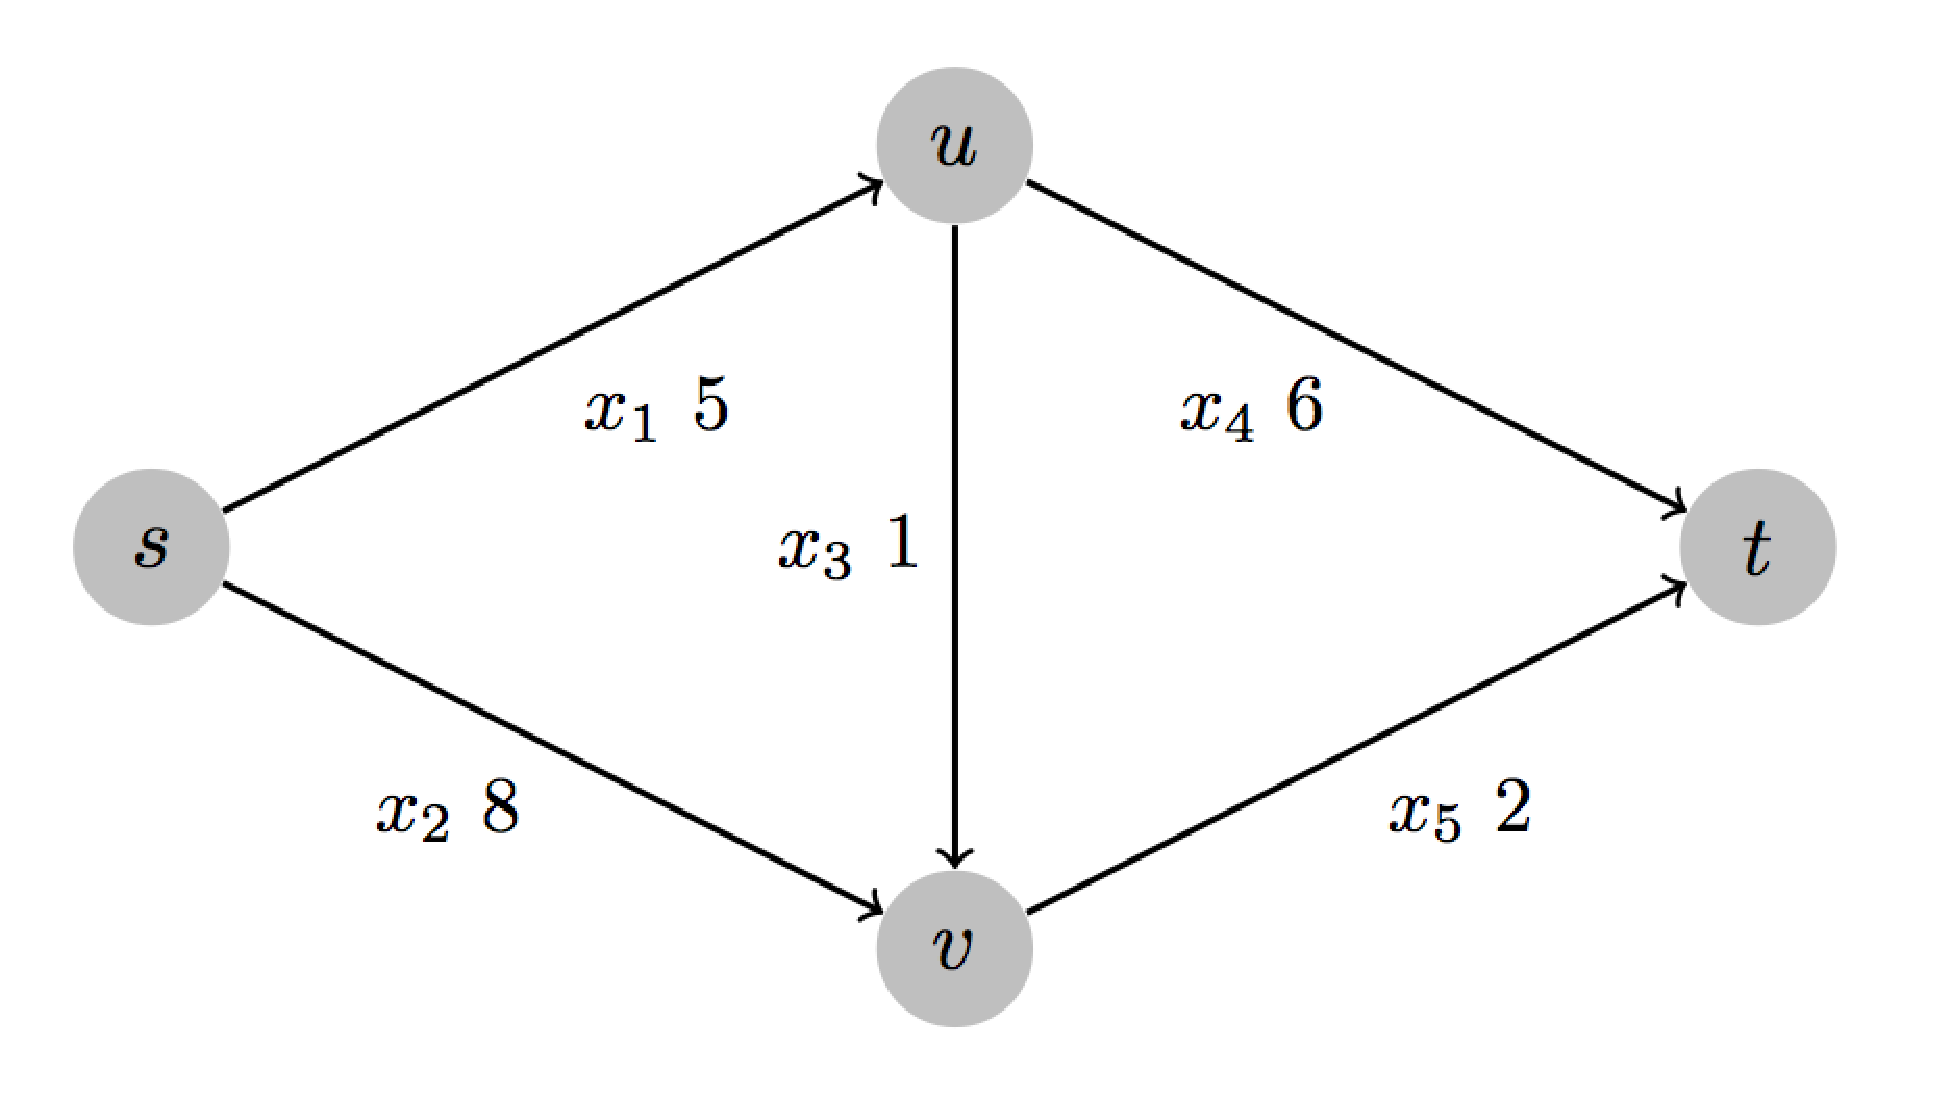
\includegraphics[width=2in]{L8-networkflowexampleLP.eps}
\end{center}


如图,假设有四个城市,s,u,v,t。连线表示,城市之间有道路。连线上的数字表示这条道路每天最多能够运送货物的吨数。比如,城市s,u之间有条路,这条路每天最多运5吨货物。

如果你是调度员,请设计一个调度方案,使得从s 到t 一天之内能够运送的货物越多越好。

现在我们形式化这个问题,将5条路的运输量分别为x1,x2,x3,x4,x5。然后写出约束条件和目标函数。

\textbf{LP Formulation:}
\[
\begin{array}{rrrrrrrrrrlr}
 \max & x_1 &+&  x_2 & &     & &     & &       & & \text{output from  } s\\
 s.t. & x_1 & &      &-& x_3 &-& x_4 & &       & = 0 & \text{node } u \\
      &     & &  x_2 &+& x_3 & &     &-&  x_5  & = 0 & \text{node } v  \\
      &     & &      & &     & &  5   &\geq &  x_1  &\geq 0 & \text{edge }  (s, u)\\
%       &     & &      & &     & &     & &  x_1  &\leq 5 &(node u)\\
      &     & &      & &     & &     & &  ...  & ... & \\
\end{array} \nonumber
\]

\textbf{注意:}因为u,v是中间节点,所以必须满足运入u,v的货物必须在当天运出。另外要满足每条路的运输量不超过其最大运量。我们的目标是要从s运出的货物越多越好。

\subsection{第三个例子:最小费用流问题}

\textbf{问题:}
%图
\newpage
\begin{figure}
   \begin{center}%
     \begin{minipage}{0.4\textwidth}%
     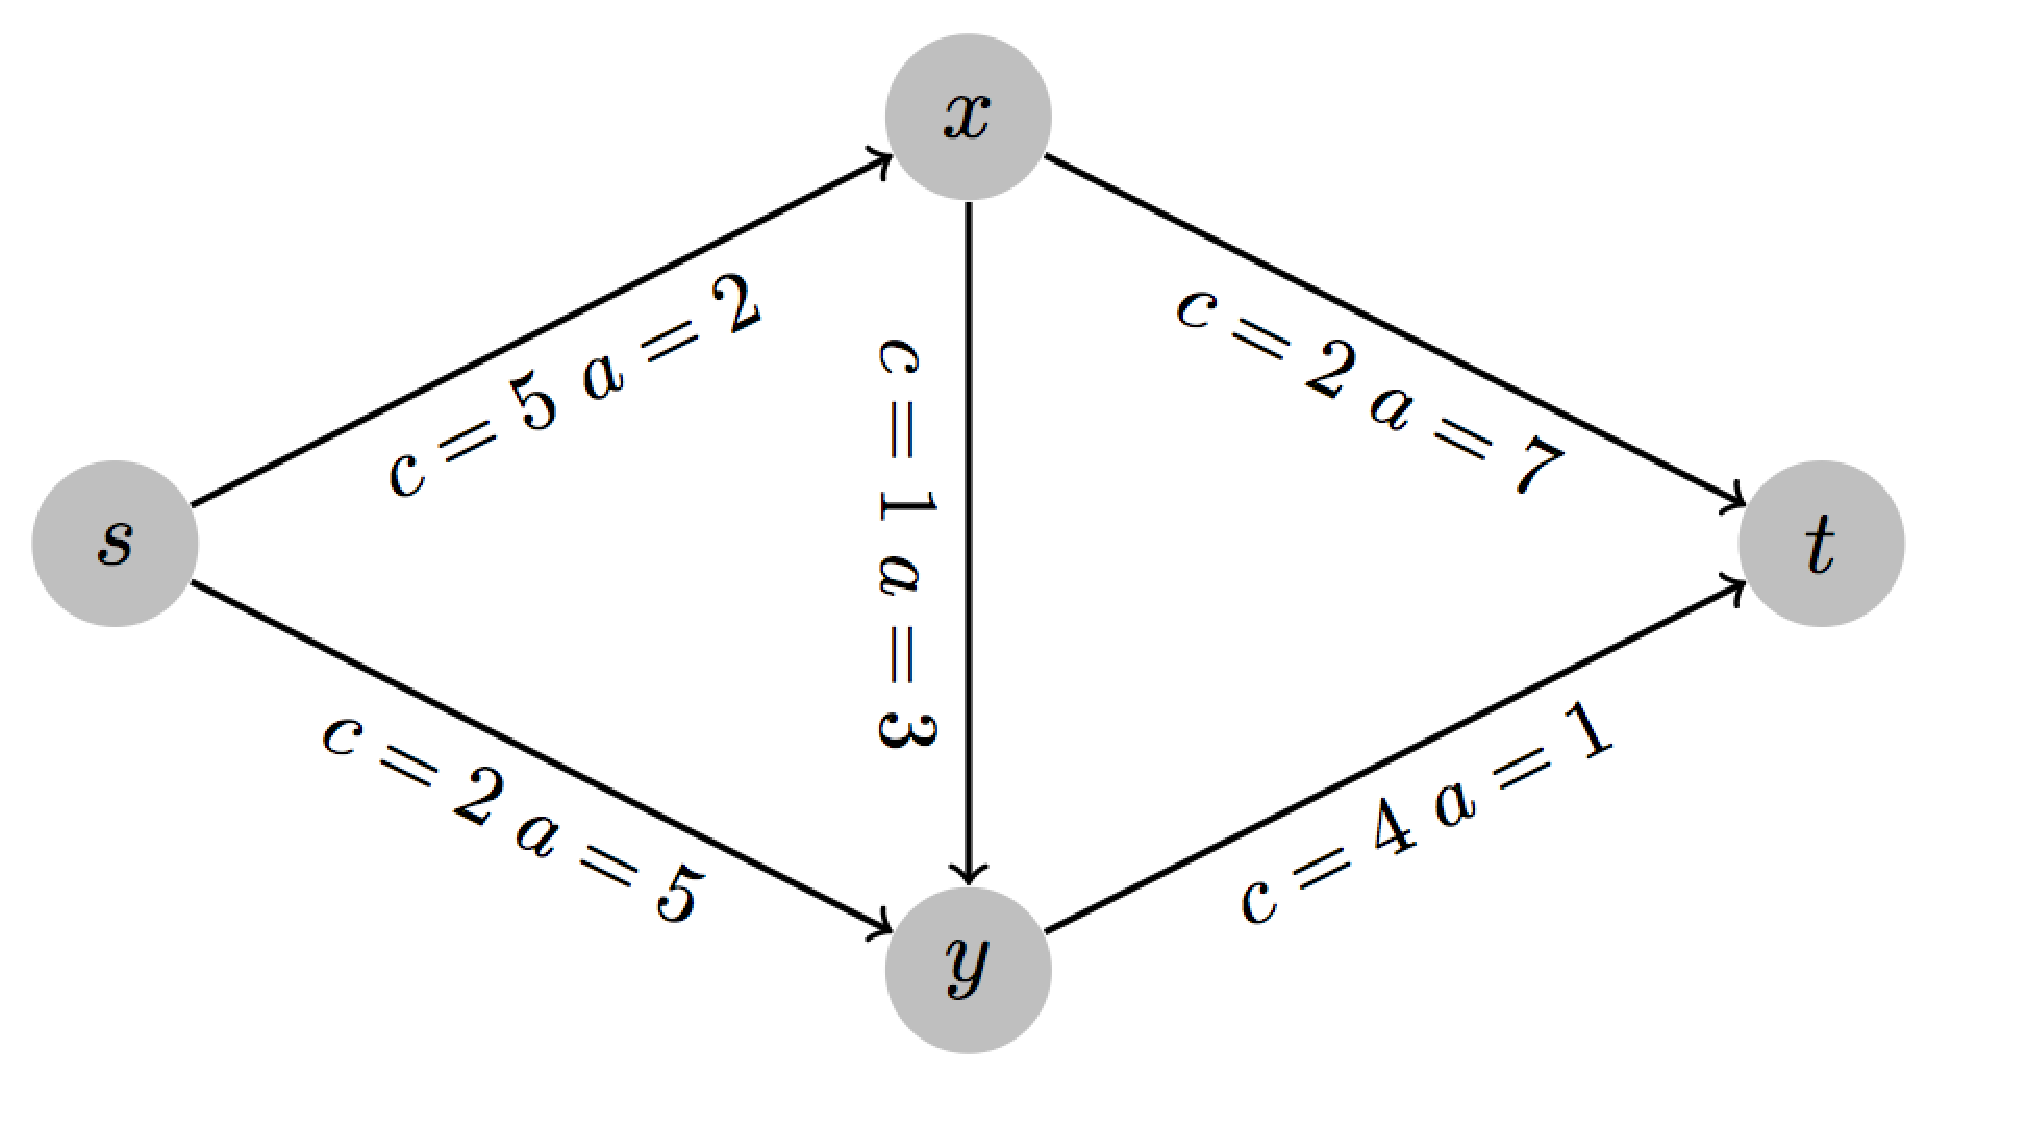
\includegraphics[width=1.0\textwidth]{L8-LPminimumcostflow1.eps}%
     \end{minipage}%
     \quad
     \begin{minipage}{0.4\textwidth}
     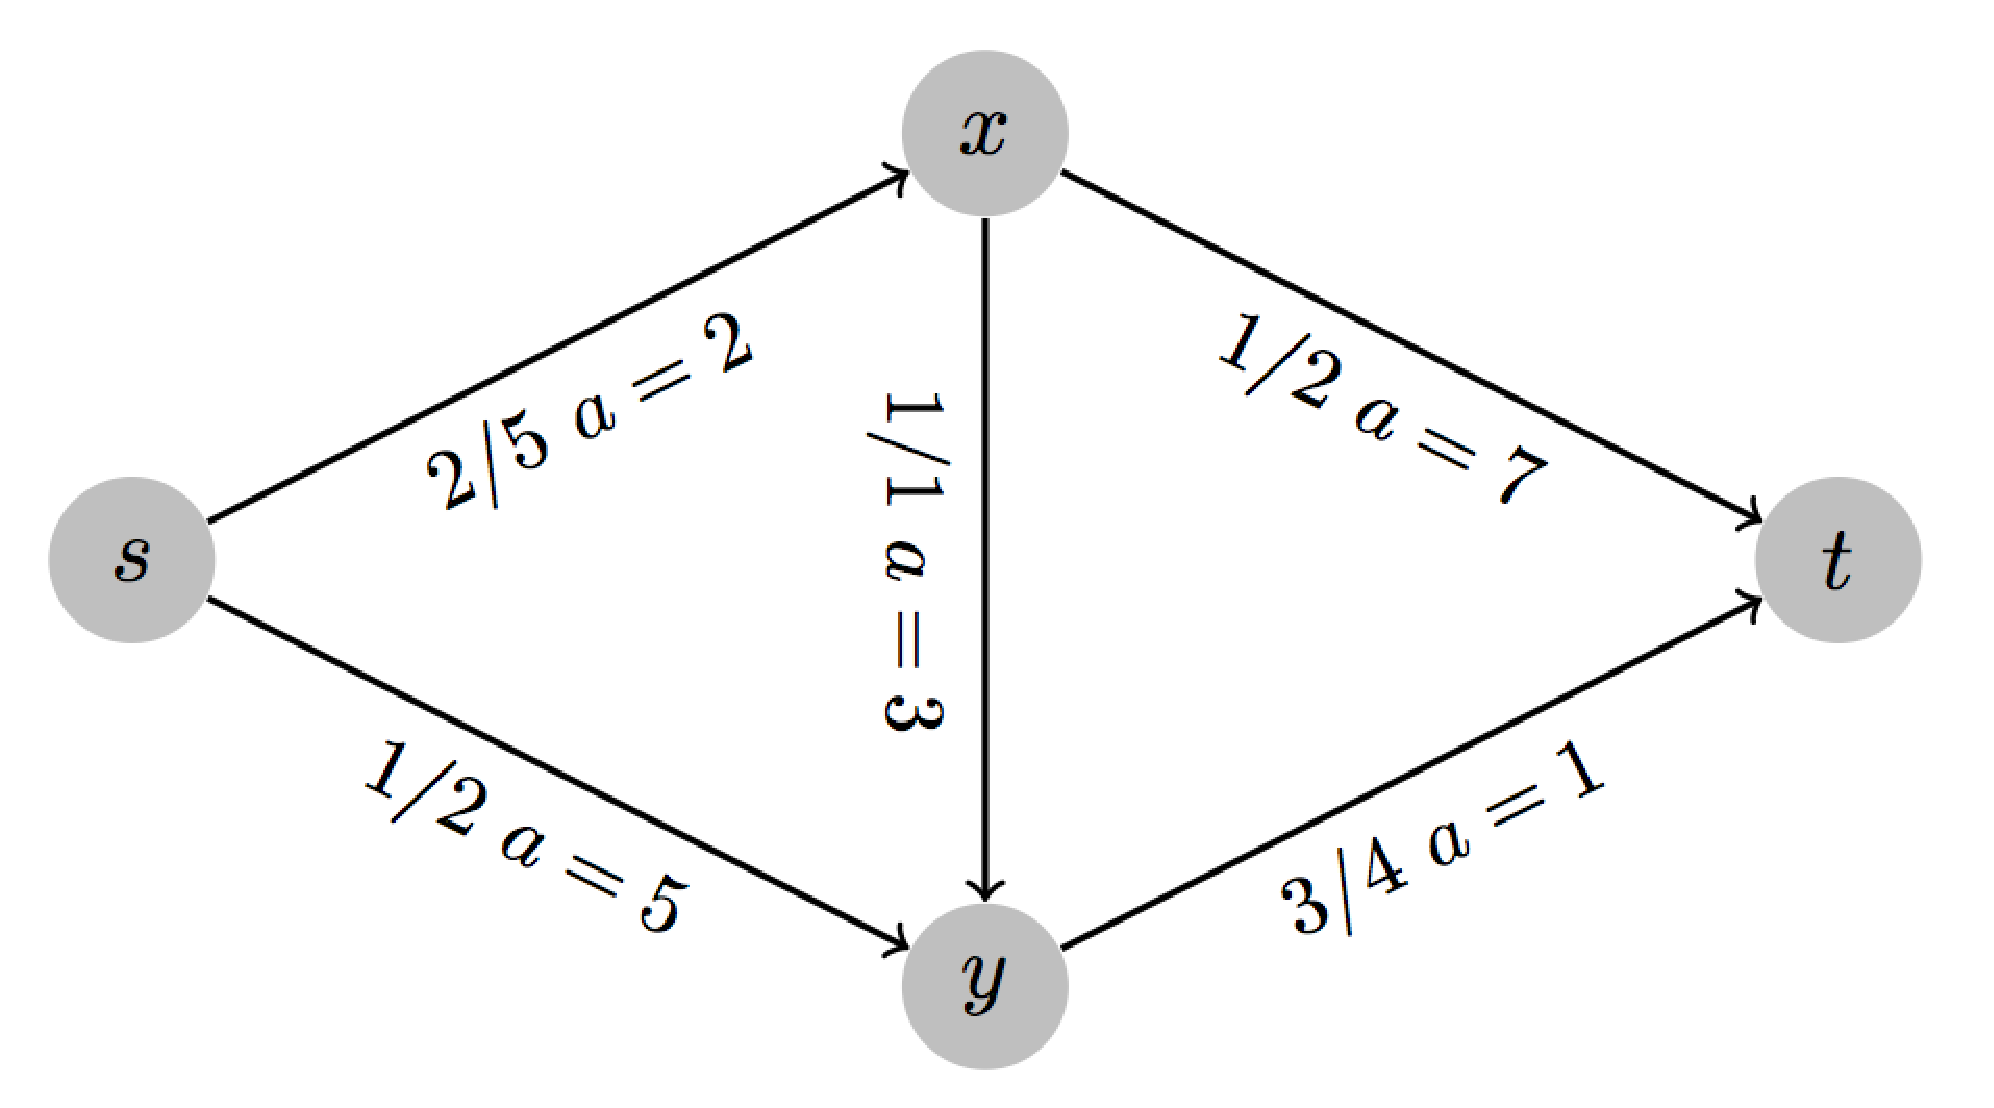
\includegraphics[width=1.0\textwidth]{L8-LPminimumcostflow2.eps}%
     \end{minipage}%
     \caption{Cost=$2\times 2 + 1\times 7 + 1\times 3 + 1\times 5 + 3\times 1 = 18$ }
   \end{center}
 \end{figure}
这个问题比刚才那个问题多了一些条件,每条路除了有最大运量的限制,另外对每条路都给出了运输每吨货物的运价。

现在有d吨的货物要从s运到t,怎样运输能使运费最少?比如上图右边的运输方案,花费为18。

下面形式化这个问题,
\textbf{LP Formulation:}
\[
\begin{array}{rrrrl}
 \min & \sum_{(u, v) \in E} a(u,v)  f(u, v)   & & & \\
 s.t. & f(u,v)   & \leq & C(u,v) & \text{for each } (u,v) \in E\\
      & f(u,v)                & \geq & 0 &  \text{for each }  (u, v) \in E\\
      & \sum_{u, (u, v) \in E} f (u,v) & = & \sum_{w, (v, w) \in E} f (v,w)  & \text{for each }  v\in V-\{s, t\}\\
%       &                         &   &   & u\in V-\{s_i, t_i\} \\
      & \sum_{v, (s, v) \in E} f( s, v) &=& d &  \\
\end{array} \nonumber
\]

\textbf{注意:}$a(u,v)$表示u到v之间的运输成本,$f(u, v)$表示u 到v 之间运送货物的吨数,$C(u,v)$ 表示u到v之间允许的最大运货量。

\subsection{第四个例子:多物品流问题}
\textbf{问题:}
\begin{center}
	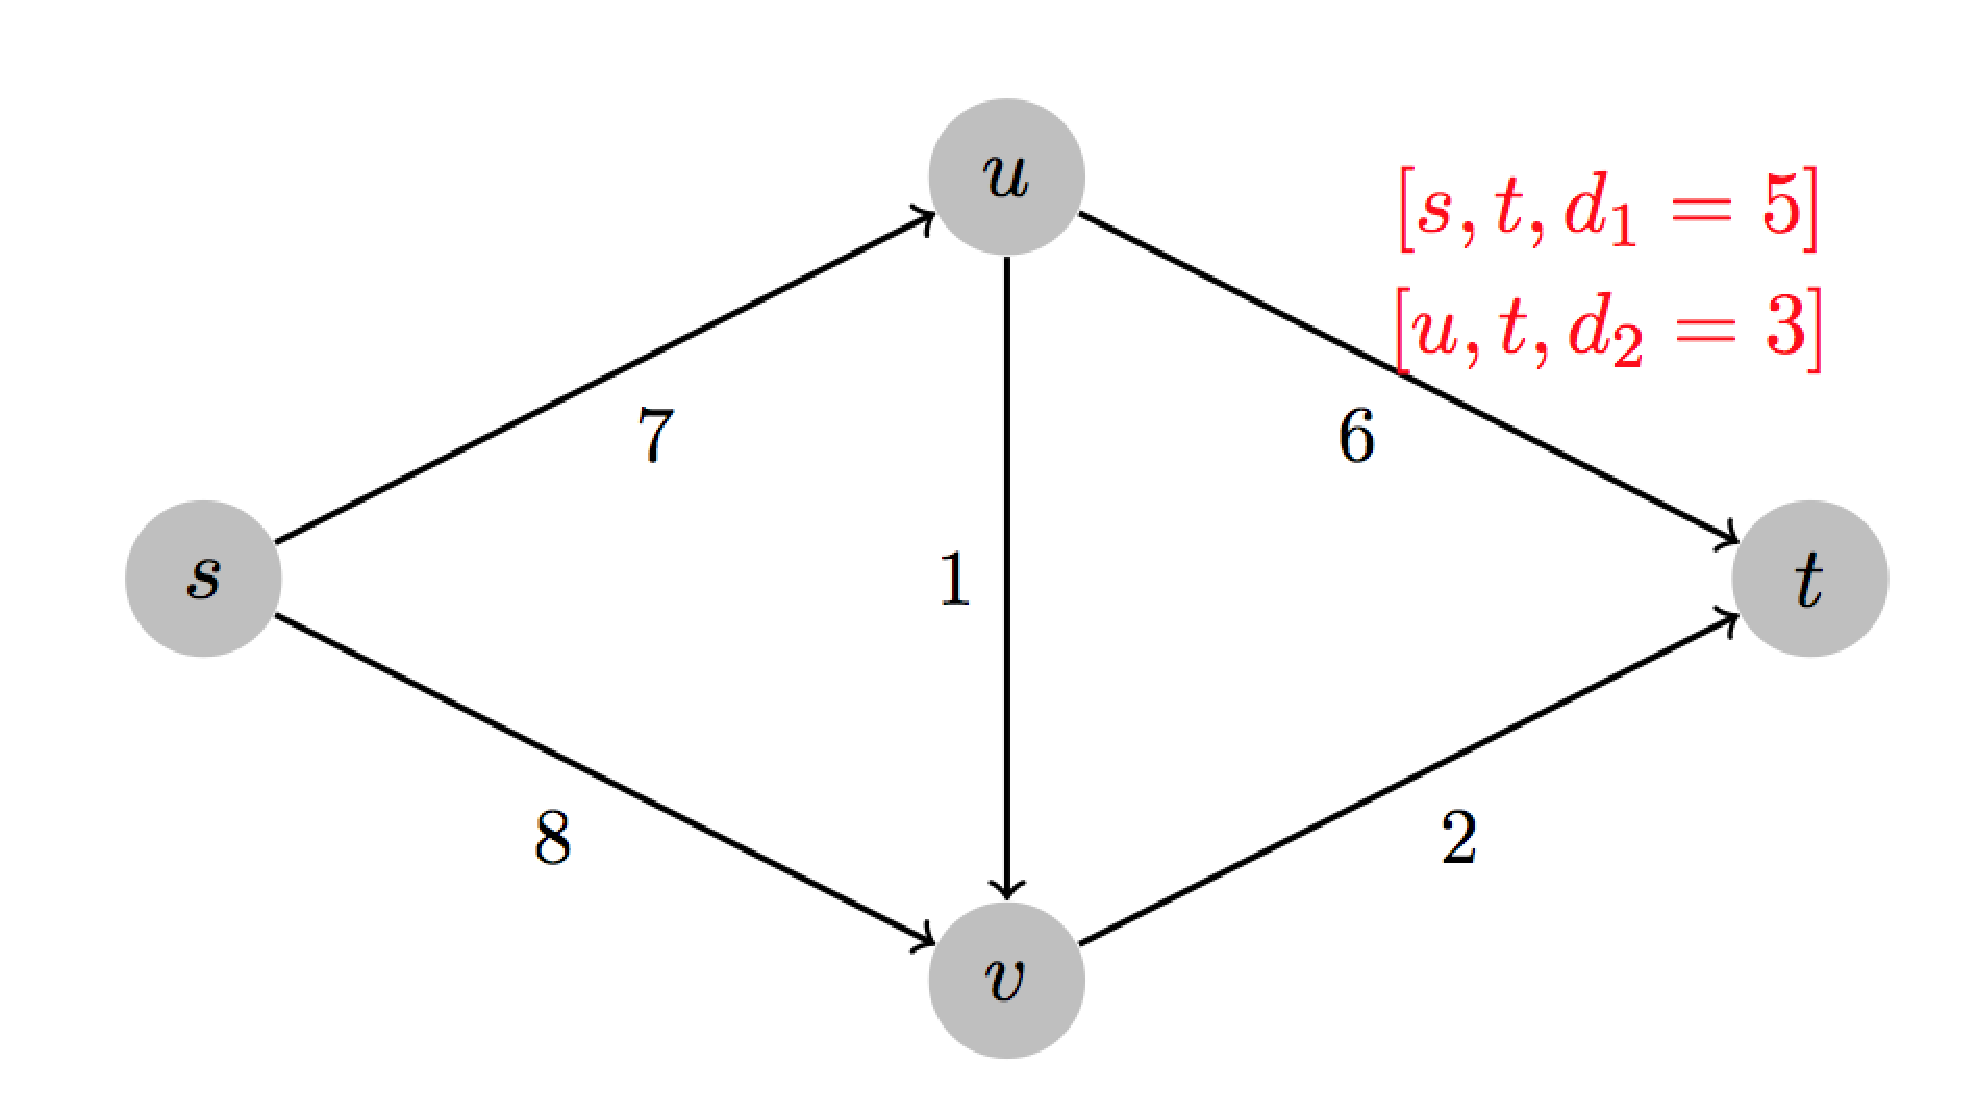
\includegraphics[width=2in]{L8-multicommodityflowexample.eps}
\end{center}


四个城市的交通网络,要从s到t运送5吨货物d1,同时要从u到t运送3 吨货物d2。这个问题与之前不同的是,要同时运送两种货物。

\textbf{LP Formulation:}
\[
\begin{array}{rrrrl}
 \max & 0   & & & \\
 s.t. & \sum_{i=1}^k f_i(u,v)   & \leq & c(u,v) & \text{for each } (u,v) \\
      & f_i(u,v)                & \geq & 0 &  \text{for each }  i, (u, v) \\
      & \sum_{u, (u, v) \in E} f_i (u,v) & = & \sum_{w, (v, w) \in E} f_i (v,w)  & \text{for each } i, v\in V-\{s_i, t_i\} \\
%       &                         &   &   & u\in V-\{s_i, t_i\} \\
      & \sum_{v, (s_i, v) \in E} f_i( s_{i}, v) &=& d_i & \text{for each }  i\\
\end{array} \nonumber
\]

\textbf{注意:}目标函数为$max  0$,这个看起来有些奇怪,其实这个问题只需要解出满足这些约束条件的解就可以了。

讲到这里我们就可以回答为什么这堂课是我们思维的一个转折点了。我们以前遇到一个问题可以分解,我们就很高兴,有很多的办法去解决,但是上面这个问题是不容易分解的。值得指出的是,线性规划是到目前为止唯一的一个多项式算法。也就是说,我们或许可以写出一个多物品的贪心算法,但它的时间复杂度不是多项式时间的。

\subsection{第五个例子:多物品流问题}

SAT问题值得讲, 因为它是一个整数线性规划问题。

\textbf{问题:}

\begin{mdframed}[leftmargin=10pt,rightmargin=10pt]
{\bf INPUT: }  \\
      A set of $m$ conjunction normal formula (CNF) clauses over $n$ Boolean variables $x_{1}, x_{2}, ..., x_{n}$ \\
     {\bf OUTPUT: } \\
      Whether all clauses can be  satisfied by an {\tt TRUE/FALSE} assignment of the $n$ variables.
\end{mdframed}

\begin{itemize}
\item
A {\sc SAT } instance:
\[
\begin{array}{rrrrl}
 \Phi & = & ( x_1 \vee \neg x_2 \vee x_3 ) & \wedge \\
      &  & ( \neg x_1 \vee  x_2 \vee \neg x_3 ) & \wedge \\
      &  & (      x_1 \vee  x_2 \vee \neg x_3 ) & \\
 \end{array} \nonumber
\]
\item
An assignment to make all clauses {\tt TRUE}:

\[
x_{1}=\texttt{TRUE}, x_{2}=\texttt{TRUE}, x_{3}=\texttt{TRUE}
\]
\end{itemize}


\textbf{注意:}每个$x_{i}$都为一个布尔变量,取值只能是TRUE或者FALSE两者之一。用$\vee$连起来的式子叫做子式,这些子式连接成一个和取范式。能不能找到一种组合,使得所有的子式都为TRUE?这个是可以做到的,比如我们取$x_{1}=\texttt{TRUE}, x_{2}=\texttt{TRUE}, x_{3}=\texttt{TRUE}$, 就可以使得三个子句都为TRUE。

对于这个问题,诸位怎样求解呢?先看能不能分解?答案是肯定的,我们下堂课介绍分解的方法。我们先来看不分解的方法,把这个问题写成下面的形式:

\textbf{LP Formulation:}
\[
\begin{array}{rrrrl}
 \max & c_1 +&  c_2 +& c_3 & \\
 s.t. & x_1 +& (1-x_2) +& x_3 & \geq c_1 \\
      & (1-x_1) +&  x_2 +& (1-x_3) & \geq c_2 \\
      & x_1 +&  x_2 +& (1-x_3) & \geq c_3 \\
      & x_1 ,& x_2 ,& x_3 & = 0/1 \\
      & c_1 ,& c_2 ,& c_3 & = 0/1
\end{array} \nonumber
\]

\textbf{注意:}第一行的$max  c_1 +  c_2 + c_3 $表明,$c_1,c_2 ,c_3$均取1。 所以对于这个例子来说,当且仅当$c_1+c_2+c_3=3$时才成立。

%\emph{也可以取另外一种赋值, ?这个地方可能写错了}

在这个问题中每个$x_{i}$只能取0或1两个值,这样的问题叫做整数线性规划。

\subsection{补充例子:基因组重排问题}
%\emph{31:30-43:48,基因组问题
\textbf{问题:}
\begin{itemize}
	\item The minimum number of operations to transform $G_1$ into $G_2$
	\end{itemize}
	\vspace{0.2cm}
	\begin{center}
		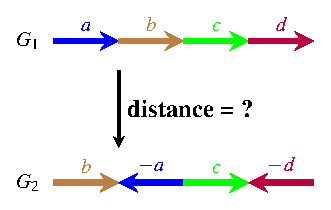
\includegraphics[width=0.6\textwidth]{mingfudistance.eps}
	\end{center}
	Operations:  reverse a fragment of the genome;


假设人的基因组$G_1$上有$a,b,c,d$这样四个基因,老鼠的基因组$G_2$上$a,d$这两个基因是反过来的,问基因组$G_1$翻转几次可以得到基因组$G_2$?

\textbf{补充:}
如果诸位熟悉计算机历史的话,这个问题是否曾经见过?这是Bill Gates退学前和老师一起研究的一个翻煎饼的问题。(这里有一个Bill 的故事和翻煎饼的说明)


\textbf{形式化模型:}
我们给这个问题建立一个邻接图形式化的模型。
\begin{center}
	\includegraphics[width=0.95\textwidth]{mingfuadjgraph.eps}
\end{center}
\begin{itemize}
	\item 可以证明: DCJ distance = (\#adjacencies) $-$ (\#cycles).
	\item 在这个例子中, DCJ distance = 3
	\item 所以在这个图中,因为adjacencies为固定值,所以求最小的DCJ distance 的问题就转换为求图中有多少个环的问题。
\end{itemize}

\textbf{问题描述:}

\vspace{-0.3cm}

	{\bf Problem:} given an undirected graph $G=(V,E)$, to choose $k$ edges and remove others,
	such that the number of connected components in the remaining graph is maximized. \\
	({\bf Formulate this problem as an ILP}.)

	\vspace{0.6cm}

	\begin{center}
	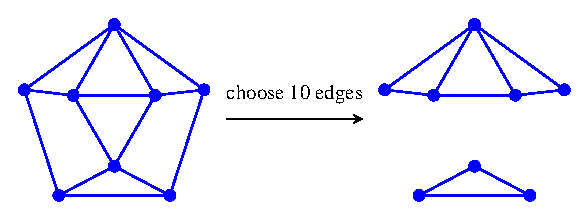
\includegraphics[width=\textwidth]{mingfustar.eps}
	\end{center}

假定要从一个图中选出一些边,使得连通的点越多越好。

\textbf{例子:}
比如我们要选出3条边,使得连通的点越多越好。

\begin{center}
	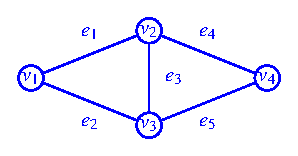
\includegraphics[width=0.5\textwidth]{mingfuexample.eps}
\end{center}

\begin{itemize}
	\item 用$x_{i}$表示第$i$条边是否被选择,选则为1,不选为0。
		\begin{displaymath}
			x_1 + x_2 + x_3 + x_4 + x_5 = 3
		\end{displaymath}
    \item 用$y_i$来表示第$i$个顶点的标签。
		\begin{eqnarray*}
			1\le  y_1  \le 1\\
			1\le  y_2  \le 2\\
			1\le  y_3  \le 3\\
			1\le  y_4  \le 4\\
		\end{eqnarray*}
    \item 如果一条边被选择,它的两个顶点需要有相同的标签。
		\begin{align*}
			y_1 \le y_2 + 1 \cdot (1 - x_1);\  y_2 \le y_1 + 2 \cdot (1 - x_1) \tag{for $e_1$}\\
			y_1 \le y_3 + 1 \cdot (1 - x_2);\  y_3 \le y_1 + 3 \cdot (1 - x_2) \tag{for $e_2$}\\
			y_2 \le y_3 + 2 \cdot (1 - x_3);\  y_3 \le y_2 + 3 \cdot (1 - x_3) \tag{for $e_3$}\\
			y_2 \le y_4 + 2 \cdot (1 - x_4);\  y_4 \le y_2 + 4 \cdot (1 - x_4) \tag{for $e_4$}\\
			y_3 \le y_4 + 3 \cdot (1 - x_5);\  y_4 \le y_3 + 4 \cdot (1 - x_5) \tag{for $e_5$}\\
		\end{align*}
    \item 同样的连通单元中的顶点有相同的标签。

	\item Since all vertices have distinct upper bounds, in each connected
	component, at most one vertex can reach its upper bound. Thus, we
	can use the number of vertices whose upper bound is reached, to count the number of connected components.
    \item<2-> We use a binary variable $z_j$ to indicate whether the label of $v_j$ reaches its upper bound:
		\begin{eqnarray*}
			1 \cdot z_1 \le y_1 \\
			2 \cdot z_2 \le y_2 \\
			3 \cdot z_3 \le y_3 \\
			4 \cdot z_4 \le y_4
		\end{eqnarray*}
	We can verify that, $z_j = 1$ only if $y_j = j$, i.e., the label of $v_j$ reaches its upper bound.
	\item The objective function of the ILP formulation can be set to maximize the number of vertices
		whose upper bound can be reached:
		\begin{displaymath}
			\max z_1 + z_2 + z_3 + z_4
		\end{displaymath}
\end{itemize}

\section{动态规划问题的历史回顾}

看了这些问题之后,大家一定会有感觉,我们生活中的很多问题,都可以写成一个最优化的问题,不论我们想要最优化的是目标函数,还是问题的约束条件,它们都是一些线性组合。这是一类很常见的问题,我们简单看一下这类问题的历史。

\subsection{问题提出:}
1946年,在美国空军的指挥部,George B. Dantzig作为数学顾问,他的同事问了他一个问题关于部队部署的问题:怎样快速调度训练计划和物流。在前电子计算机的时代,人们是用穿孔卡和一些模拟的设备来制造机械式的计算机器。"program"这个词用来表示规划和调度,而不是现在所说的编程。在1947 年,Dantzig 把这个问题抽象成了一个数学问题。

\subsection{ 有关算法和分析:}
1949 年,Dantzig又提出了单纯形算法。
大家回忆一下我们第一堂课就讲过的,解决一个问题的三个步骤。首先我们要确定要解决的实际的问题是什么,然后将它用公式描述为一个数学问题,最后提出算法。Dantzig 的这个故事向我们清晰的展示了这三个步骤,首先在1946年他的同事向他提出了这个问题,1947年他为这个问题建立了数学模型,然后在1949 年,他提出了解决这个问题的单纯形算法(simplex algorithm)。

人们发现单纯形算法太好了,运行的飞快,所有的问题都解决的非常好。所以人们一直以为这个算法是多项式时间复杂度的算法,然而很不幸,在1971年,Klee 和 Minty 提出了第一个反例,说明单纯型算法不是多项式时间复杂度。这下大家产生了怀疑,线性规划问题应该是一个难以分解(NP hard)的问题,因为单纯型算法的成功,很多人都在用它。典型的例子是,1975 年L. V. Kantorovich 和 T. C. Koopmans将线性规划的方法用于经济学领域的资源分配问题上,得到了诺贝尔经济学奖。

在1971年后,虽然人们怀疑线性规划问题是NP完全问题,但是在1979年,峰回路转,苏联科学家 L. G. Khanchian提出了多项式时间复杂度的椭球算法,这是一个可以分解的问题。椭球法理论上非常漂亮,常常用于其他领域,但是实际效果却很慢,不实用。1984年,另一个苏联科学家 N. Karmarkar提出了内联法,是多项式时间复杂度的算法,同时运行起来也非常快。

但是这个问题还是没有完全解决,人不不知道为什么单纯型算法理论上是指数型复杂度,但实际运行时却常常是多项式时间复杂度。直到2001 年,D. Spielman和S. Teng 提出了平滑型复杂度理论(smoothed complexity),完美地证明了这个问题。

\subsection{NLP, Convex Programming, LP, Network flow, 和 ILP:}

\begin{center}
	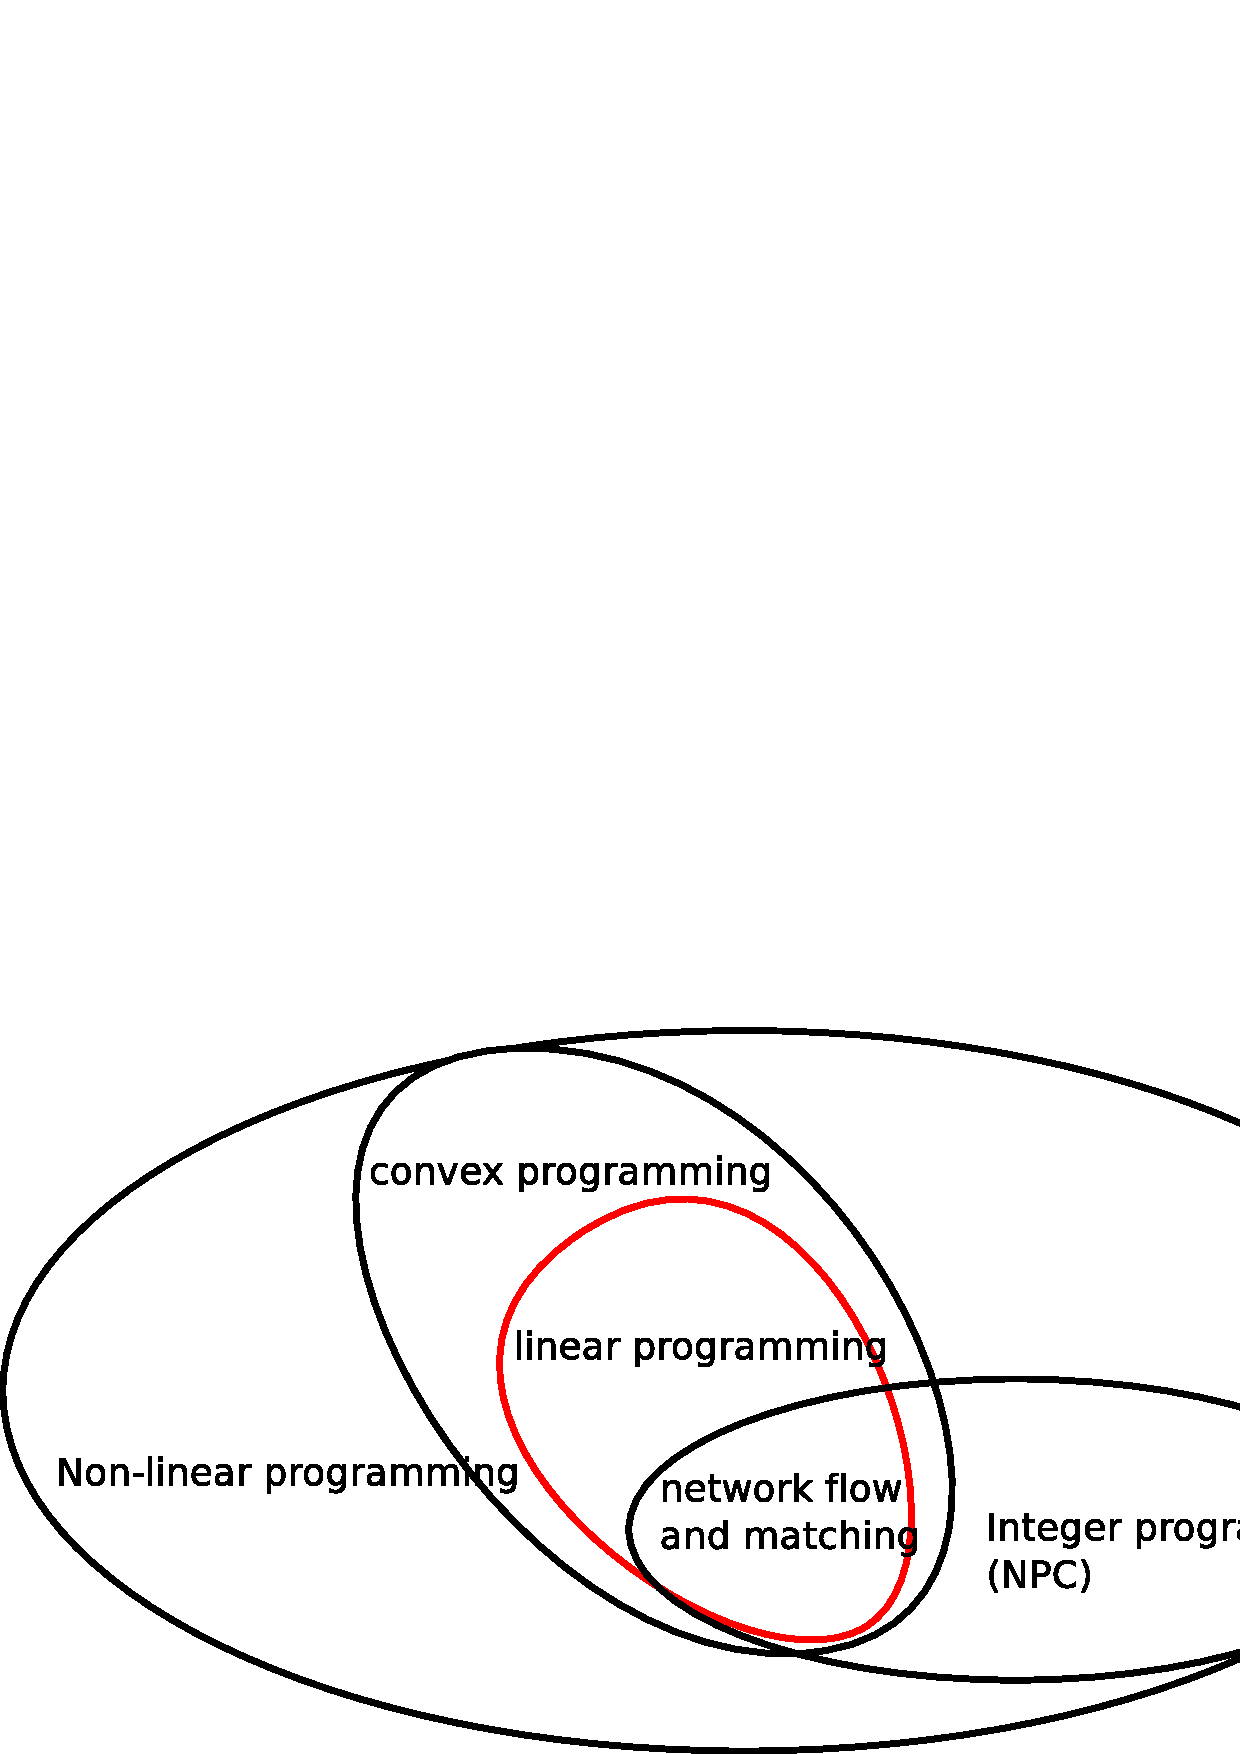
\includegraphics[width=0.95\textwidth]{L8-NLPLP.png}
\end{center}

我们发现生活中的很多问题都能够描述成一个优化的问题,诸位以后研究生生涯中碰到的问题可能80\%的情况是优化问题,所以最外面这个大圈,就可以覆盖大家研究问题80\%的情况。这里面有一类凸的规划是非常特殊的,目标函数是凸的,可行域也是凸的,这就是凸规划问题。凸规划问题里面又有一个线性规划问题,目标函数和约束都是线性组合。还有另一类问题是整数型规划问题,我们学过的网络流和匹配这两类问题是整数型规划问题,但是它们又很特殊,网络流问题中假设$ 0 \leq x_{i} \leq 1 $,但是线性规划问题$ x_{i} $只有0或1两种取值。

\subsection{求解LP问题的工具:}
现在有很多求解线性规划的软件包,典型的一个包是GLPK,还有一个是Gurobi,是目前运行最快的软件包。下面给大家看两个例子:

\emph{55:25-第一部分结束,演示}

\section{线性规划问题的求解}

前面介绍了建模的方法,下面介绍求解的过程。

线性规划问题的形式有:一般形式,标准形式和松弛形式。

\subsection{一般形式线性规划问题}
\begin{itemize}
\item
General form: mixture of linear inequalities and equalities
\[
\begin{array}{rrrrrrrrrrrrl}\nonumber
 \min & c_1x_1    &+&  c_2x_2   &+&  ...&+& c_nx_n    &      &     & \\
 s.t. & a_{i1}x_1 &+& a_{i2}x_2 &+& ... &+& a_{in}x_n & \geq & b_i & i \in M\\
      %&           & &           & & ... & &           &        &          &\\
      & a_{j1}x_1 &+& a_{j2}x_2 &+& ... &+& a_{jn}x_n &  =   & b_j & j \in \overline{M} \\
      &           & &           & &     & &       x_i & \geq & 0   & i \in N
 %     &           & &           & &     & &       x_j &\leq\geq & 0 & j \in \overline{N} \\
     \end{array} \nonumber
\]
\end{itemize}

\subsection{标准形式线性规划问题}
\begin{itemize}
 \item
Standard form: linear inequalities;
\[
\begin{array}{rrrrrrrrrrrrl}
 \min & c_1x_1    &+&  c_2x_2   &+&  ...&+& c_nx_n    &      &    & \\
 s.t. & a_{11}x_1 &+& a_{12}x_2 &+& ... &+& a_{1n}x_n & \textcolor{red}{\leq} & b_1 &  \\
      & a_{21}x_1 &+& a_{22}x_2 &+& ... &+& a_{2n}x_n & \textcolor{red}{\leq} & b_2 &  \\
      &   ...    & &   ...   & & ... & & ... &      &     &  \\
      & a_{m1}x_1 &+& a_{m2}x_2 &+& ... &+& a_{mn}x_n & \textcolor{red}{\leq} & b_m &  \\
      &           & &           & &     & &       x_i & \geq & 0   & \text{for } \forall i
     \end{array} \nonumber
\]
\item


Standard form in matrix language:
\[
\begin{array}{rrrrrrrrrrrrl}
 \min & \mathbf{c^Tx}   \\
 s.t. & \mathbf{Ax \leq b} \\
      & \mathbf{x \geq 0} \\
\end{array} \nonumber
\]

\item Here
$\mathbf{c} = \left(
	   \begin{array}{c}
		 c_1 \\
	  	        c_2\\
	                                \vdots \\
	                         c_n
	      \end{array}
	      \right) $,
	$\mathbf{x} = \left(
	   \begin{array}{c}
		 x_1 \\
	  	        x_2\\
	                                \vdots \\
	                         x_n
	      \end{array}
	      \right) $, \\
			      $\mathbf{A}=\left(
	\begin{array}{cccc}
	a_{11} & a_{12} & \cdots & a_{1n} \\
	a_{21} & a_{22} & \cdots & a_{2n} \\
	\vdots & \vdots & \ddots & \vdots \\
	a_{m1} & a_{m2} & \cdots & a_{mn}
	\end{array}
	\right)$,
	$\mathbf{b} = \left(
	   \begin{array}{c}
		 b_1 \\
	  	        b_2\\
	                                \vdots \\
	                         b_m
	      \end{array}
	      \right) $.

\end{itemize}

\textbf{注意:}在一般形式的线性规划问题中,约束条件函数可能有等式和不等式的形式,我们希望把这些约束条件统一写成标准的方程形式,比如都写成用$\leq$ 表示的方程,并且满足$x_{i} \geq 0 $。我们做如下变换:

\textbf{一般形式转换为标准形式:}
\begin{itemize}
\item  Transformations:
\begin{enumerate}
\item \textcolor{red}{\bf Variables:}  a free variable $\Rightarrow$  two non-negativeive variables; \\
$x_i$ may or may not be positive  $\Rightarrow$  replacing $x_i$ with $x_i' - x_i''$ \\
     and adding constraints: $x_i' \geq 0 ; x_i'' \geq 0$
\ \\
\ \\
 \item \textcolor{red}{\bf Constraints:}  an equality $\Rightarrow$ two inequalities; \\
 $a_{j1}x_1 + a_{j2}x_2 + ... + a_{jn}x_n  \textcolor{red}{=}  b_j \Rightarrow $\\
$a_{j1}x_1 + a_{j2}x_2 + ... + a_{jn}x_n  \textcolor{red}{\geq} b_j $\\
$a_{j1}x_1 + a_{j2}x_2 + ... + a_{jn}x_n  \textcolor{red}{\leq} b_j $
\end{enumerate}
\end{itemize}

\subsection{松弛形式线性规划问题}
\begin{itemize}
\item
Slack form: linear equality;
\[
\begin{array}{rrrrrrrrrrrrl}
 \min & c_1x_1    &+&  c_2x_2   &+&  ...&+& c_nx_n    &      &    & \\
 s.t. & a_{11}x_1 &+& a_{12}x_2 &+& ... &+& a_{1n}x_n & \textcolor{red}{=} & b_1 &  \\
      & a_{21}x_1 &+& a_{22}x_2 &+& ... &+& a_{2n}x_n & \textcolor{red}{=} & b_2 &  \\
      &  ... & &   ... & & ... & &  ...  &      &     &  \\
      & a_{m1}x_1 &+& a_{m2}x_2 &+& ... &+& a_{mn}x_n & \textcolor{red}{=} & b_m &  \\
      &           & &           & &     & &       x_i & \geq & 0   & \text{for } \forall i
     \end{array} \nonumber
\]
\item
Slack form in matrix language:
\[
\begin{array}{rrrrrrrrrrrrl}
 \min & \mathbf{c^Tx}   \\
 s.t. & \mathbf{Ax = b} \\
      & \mathbf{x \geq 0} \\
\end{array} \nonumber
\]
\end{itemize}

\textbf{注意:}松弛形式也是一种比较常见的形式,所有的约束条件方程都采用等式的形式。假如一开始我们写出的目标函数是$a_{j1}x_1 + a_{j2}x_2 + ... + a_{jn}x_n  \textcolor{red}{  \leq } b_j$的形式,可以引入一个整数$s$,使之变为等式形式,$s$称为松弛变量。

\begin{itemize}
\item
Transformations:
\begin{enumerate}
 \item
\textcolor{red}{\bf Variables:} changing ``inequality on partial solution $(x_1,...,x_n)$'' to ``equality on full solution $(\textcolor{red}{s}, x_1, ..., x_n)$'' by introducing a slack variable $s$. \\
$a_{j1}x_1 + a_{j2}x_2 + ... + a_{jn}x_n  \textcolor{red}{  \leq } b_j \Rightarrow $\\
$a_{j1}x_1 + a_{j2}x_2 + ... + a_{jn}x_n  \textcolor{red}{ + s = } b_j $\\
\ \\
\ \\
\item
\textcolor{red}{\bf Constraint:}  $s \geq 0 $.  ($s$ is called a slack variable)
\end{enumerate}
\end{itemize}

\textbf{例子:标准形式 VS 松弛形式}
\begin{itemize}
\item
Standard form:
\[
\begin{array}{rrrrrrrrrrrrl}
            & &             &-&x_3     &+&2x_4  & \textcolor{red}{\leq} & 2 &  \\
             & &           & & 3x_3  &-&2x_4  &  \textcolor{red}{\leq} & 6 &  \\
        & &  & & x_{3}&,&x_{4} &  \geq  & 0 & \\
     \end{array} \nonumber
\]

\item
Slack form:
\[
\begin{array}{rrrrrrrrrrrrl}
     \textcolor{red}{  x_1 }& &             &-& x_3     &+&2x_4  & \textcolor{red}{=} & 2 &  \\
             & & \textcolor{red}{  x_{2} }   &+& 3x_3  &-&2x_4  &\textcolor{red}{=}& 6 &  \\
      \textcolor{red}{ x_1} &,& \textcolor{red}{ x_2} &,& x_{3}&,&x_{4} &  \geq  & 0 & \\
     \end{array} \nonumber
\]
\end{itemize}

\textbf{注意:}大家不要小看这种变换,把不等式的约束变为等式的约束,是线性规划中常常要考虑的问题。

\subsection{求解方法}
下面我们讨论怎样求解。
\[
\begin{array}{rrrrl}
 \max & c_1 +&  c_2 +& c_3 & \\
 s.t. & x_1 +& (1-x_2) +& x_3 & \geq c_1 \\
      & (1-x_1) +&  x_2 +& (1-x_3) & \geq c_2 \\
      & x_1 +&  x_2 +& (1-x_3) & \geq c_3 \\
      & x_1 ,& x_2 ,& x_3 & = 0/1 \\
      & c_1 ,& c_2 ,& c_3 & = 0/1
\end{array} \nonumber
\]

\textbf{方法一:}
首先观察解的形式,$\mathbf{X = [x_1, x_2, x_3, x_4]} (x_i = o/1)$,一定可以画出一个部分解的枚举树,叶子节点即为所求的完整解。如下:

\begin{itemize}
		\item Solution: $X=[x_1, x_2, ..., x_n]$, $x_i = 0/1$
		\item Partial solution enumeration tree:
	\begin{center}
		\includegraphics[width=0.6\textwidth]{Branch-and-bound1.png}
	\end{center}
		\item We will talk about ``intelligent enumeration", say branch-and-bound, and backtracking, later.
	\end{itemize}

\textbf{注意:}我们的目标就是从8个完整解中找出最好的解。另外除了使用枚举的方法,贪心法,回溯法,分支限界法均可以使用。所以,我们的解题思路是,只要解的形式为$\mathbf{X = [x_1, x_2, x_3, x_4]} (x_i = o/1)$,就可以使用各种方法来找最优解。

\textbf{扩展:}如果$x_i \subset [0,1]$,我们可以用分支限界的方法。分支限界实际上就是枚举,只不过要枚举的聪明一点,要进行大幅度的剪支,加快运行速度。这种方法会在后续学习中讨论。

\textbf{方法二:}
我们换一种思路,考虑完全解的情况。我们不对问题进行分类,也不对解进行分类,每次都考虑完整的解。画出解空间如下,

\begin{center}
		\includegraphics[width=0.6\textwidth]{ImprovementStrategy.png}
\end{center}

每个格子点都是一个完整解,如果两个格子点之间X的距离如果非常小,表示对一个解进行很小的改变就可以到达另一个解。

%12:20开始
\subsection{线性规划问题的直观认识}
我们讨论第二种求解方法,每次都考虑完整解的情况。考察一个线性规划如下,
\[
\begin{array}{rrrrrrrrrrrrl}
 \min & \mathbf{c^Tx}   \\
 s.t. & \mathbf{Ax = b} \\
      & \mathbf{x \geq 0 }\\
\end{array} \nonumber
\]

大家观察一下会发现,我们已经学过如何求解$\mathbf{Ax=b}$,但没有学过优化$\mathbf{c^Tx}$,另外还要考虑$\mathbf{x \geq 0 }$这个约束条件。下面我们分别来讨论。

\subsection{约束条件$\mathbf{x \geq 0 }$的影响:}
\subsubsection{回顾线性方程$\mathbf{Ax=b}$ 的求解:}
\[
\begin{array}{rrrrrrrrrrrrl}
      x_1 & &             &-& x_3     &+&2x_4  & \textcolor{red}{=} & 2 &  \\
             & & x_{2}    &+& 3x_3  &-&2x_4  &\textcolor{red}{=}& 6 &  \\
       2x_1     &+ & x_{2}    &+& x_3  &+&2x_4  &\textcolor{red}{=}& 10 &
     \end{array} \nonumber
\]
通过高斯消元法,我们得到:
\[
\begin{array}{rrrrrrrrrrrrl}
      x_1 & &             &-& x_3     &+&2x_4  & \textcolor{red}{=} & 2 &  \\
             & & x_{2}    &+& 3x_3  &-&2x_4  &\textcolor{red}{=}& 6 &  \\
     \end{array} \nonumber
\]

4个未知量,两个方程,我们只能确定两个独立变量,得到的解平面上的任意一个点都是这个方程组的完整解。如下图:
\begin{center}
	\includegraphics[width=2in ]{L8-LEexample.png}
\end{center}


\subsubsection{约束条件$\mathbf{x \geq 0 }$ 的影响:}
下面我们考虑对这个线性方程加一个约束条件,
\begin{itemize}
\item 例如: $\mathbf{Ax=b, x\geq 0}$
\[
\begin{array}{rrrrrrrrrrrrl}
      x_1 & &             &-& x_3     &+&2x_4  & \textcolor{black}{=} & 2 &  \\
             & & x_{2}    &+& 3x_3  &-&2x_4  &\textcolor{black}{=}& 6 &  \\
       2x_1     &+ & x_{2}    &+& x_3  &+&2x_4  &\textcolor{black}{=}& 10 &  \\
              \textcolor{red}{x_1} &\textcolor{red}{,}& \textcolor{red}{x_2}&\textcolor{red}{,}& \textcolor{red}{x_{3}}&\textcolor{red}{,}&\textcolor{red}{x_{4}} &  \geq  & \textcolor{red}{0} & \\
     \end{array} \nonumber
\]
\item 通过高斯消元法,我们得到:
\[
\begin{array}{rrrrrrrrrrrrl}
      x_1 & &             &-& x_3     &+&2x_4  & \textcolor{black}{=} & 2 &  \\
             & & x_{2}    &+& 3x_3  &-&2x_4  &\textcolor{black}{=}& 6 &  \\
              \textcolor{red}{x_1} &\textcolor{red}{,}& \textcolor{red}{x_2}&\textcolor{red}{,}& \textcolor{red}{x_{3}}&\textcolor{red}{,}&\textcolor{red}{x_{4}} &  \textcolor{red}{\geq}  & \textcolor{red}{0} & \\
     \end{array} \nonumber
\]
\item 得到一个线性不等式组:
\[
\begin{array}{rrrrrrrrrrrrl}
            & &             &-& x_3     &+&2x_4  & \textcolor{blue}{\bf \leq} & 2 &  \\
             & &           & & 3x_3  &-&2x_4  &  \textcolor{blue}{\bf \leq} & 6 &  \\
             & & & & \textcolor{red}{x_{3}}&\textcolor{red}{,}&\textcolor{red}{x_{4}} &  \textcolor{red}{\geq}  & \textcolor{red}{0} & \\
     \end{array} \nonumber
\]
\end{itemize}
\begin{center}
  \includegraphics[width=2in]{L8-LP-GE.png}%
\end{center}

对于这个线性不等式组,分别画出$x_3 + 2x_4  = 2$和$3x_3 - 2x_4 = 6$之后,就可以确定出它的解域如上图的阴影区域。与刚才的平面解域不同,这个解域为多胞形。
%1052行 18:36
\subsubsection{多胞形 $\Leftrightarrow$ 可行域}

\textbf{定理:}
\textcolor{red}{\bf Any polytope}$\mathbf{P} \subset \mathbf{R}^{n-m}$ corresponds to the feasible region of a linear program $\mathbf{Ax=b, x\geq 0}$ (denoted as $F=\{\mathbf{x: Ax=b, x\geq 0 } \}$), and vice versa.

在空间$\mathbf{R}^{n-m}$中,任何一个多胞形都对应着$\mathbf{Ax=b, x\geq 0}$的一个可行域$F=\{\mathbf{x: Ax=b, x\geq 0 } \}$),反之亦然然。

也就是说,等式约束条件:$x_2 + 3x_3  - 2x_4  \textcolor{blue}{=}  6$,等价为不等式约束条件$ 3x_3  - 2x_4  \textcolor{blue}{\leq}  6$。

下面我们证明一下这个定理。

\textbf{证明:}

\textbf{注意:}变量数为n,约束条件有m个。

\textbf{Proof: feasible region $\Rightarrow$ polytope:}
\begin{itemize}
\item
Consider a \textcolor{red}{\bf feasible full solution  $\mathbf{x}$ } of the following LP:
\begin{small}
\[
\begin{array}{rrrrrrrrrrrrl}
   & a_{11}x_1 &+& a_{12}x_2 &+& ... &+& a_{1n}x_n & = & b_1 &  \\
   & a_{21}x_1 &+& a_{22}x_2 &+& ... &+& a_{2n}x_n & = & b_2 &  \\
   &           & &           & & ... & &           &      &     &  \\
   & a_{m1}x_1 &+& a_{m2}x_2 &+& ... &+& a_{mn}x_n & = & b_m &  \\
   & x_1 &,& x_2 &,& ... &,& x_n & \geq & 0 &  \\
\end{array} \nonumber
\]
\end{small}
\item
一定可以使用高斯消元法化简为:
\begin{small}
\[
\begin{array}{rrrrrrrrrrrrrrrrrl}
   & x_1 & &     & &     &+& a_{1,m+1}'x_{m+1} &+& ... &+& a_{1n}'x_n & = & b_1' &  \\
   &     & & x_2 & &     &+& a_{2,m+1}'x_{m+1} &+&... &+& a_{2n}'x_n & = & b_2' &  \\
   &     & &  ...& &     & & ... & &           &      &     &  \\
   &     & &     & & x_m &+& a_{m,m+1}'x_{m+1}&+&... &+& a_{mn}'x_n & = & b_m' &  \\
   & x_1 &,& x_2 &,& x_m &,& x_{m+1}&,&... &,& x_n & \geq & 0 &  \\
\end{array} \nonumber
\]
\end{small}


\item
By \textcolor{red}{\bf removing  positive variables $x_1, x_2,..., x_m$}, we have the following \textcolor{red}{\bf linear inequalities}:
\[
\begin{array}{rrrrrrrrrrrrrrrrrl}
    a_{1,m+1}'x_{m+1} &+& ... &+& a_{1n}'x_n & \textcolor{blue}{\bf \leq} & b_1' &  \\
   a_{2,m+1}'x_{m+1} &+&... &+& a_{2n}'x_n & \textcolor{blue}{\bf \leq} & b_2' &  \\
    & &   ...        &      &     &  \\
    a_{m,m+1}'x_{m+1}&+&... &+& a_{mn}'x_n & \textcolor{blue}{\bf \leq} & b_m' &  \\
    x_{m+1}&,&... &,& x_n & \geq & 0 &  \\
\end{array} \nonumber
\]
\item Define  a polytope $\mathbf{P} \subset \mathbf{R}^{n-m}$  as the intersection of $m$ half-spaces:

$HS_j: a_{j,m+1}'x_{m+1} + ... + a_{jn}'x_n \textcolor{blue}{\bf \leq } b_j' $ , $1\leq j \leq m$. (by $x_j \geq 0$)

\item
Thus,  \textcolor{red}{\bf any feasible full solution }  $\mathbf{x} = (x_1, x_2, ..., x_n)$   $\Rightarrow$ \textcolor{red}{\bf partial  solution  } $ \mathbf{{x}_{N}}=(x_{m+1}, ..., x_n)\in \mathbf{P}$.
\end{itemize}

\textbf{Proof: polytope $\Rightarrow$  feasible region:}

\textbf{注意:}反过来,我们加入一个松弛变量$s_j$,将一个多胞形变成了$AX=B$的形式。

\begin{itemize}
\item
Basic idea:  changing \textcolor{red}{\bf inequality} to \textcolor{red}{\bf equality} through introducing \textcolor{red}{\bf slack variables.}  \\

\begin{itemize}
 \item

Suppose $P$ is the intersection of $m$ half-spaces (inequalities), say:

$HS_j: a_{j1}x_1 + a_{j2}x_2 + ... + a_{jn}x_n \textcolor{blue}{ \leq } b_j $ ($1\leq j \leq m$)\\
\item Introducing a non-negative slack variable $s_j$ to each inequality, we have:\\
$\ \ \ \ \ \ a_{j1}x_1 + a_{j2}x_2 + ... + a_{jn}x_n +\textcolor{blue}{ s_j  = } b_j $ ($s_j \geq 0$)  \\

\end{itemize}
\end{itemize}
\begin{itemize}
\item Thus we change
\[
\begin{array}{rrrrrrrrrrrrl}
   & a_{11}x_1 &+& a_{12}x_2 &+& ... &+& a_{1n}x_n & \textcolor{blue}{\leq} & b_1 &  \\
   & a_{21}x_1 &+& a_{22}x_2 &+& ... &+& a_{2n}x_n & \textcolor{blue}{\leq} & b_2 &  \\
   &           & &           & & ... & &           &      &     &  \\
   & a_{m1}x_1 &+& a_{m2}x_2 &+& ... &+& a_{mn}x_n & \textcolor{blue}{\leq} & b_m &  \\
   & x_1 &,& x_2 &,& ... &,& x_n & \geq & 0 &  \\
\end{array} \nonumber
\]

into
\[
\begin{array}{rrrrrrrrrrrrrrrrrl}
   &\textcolor{blue}{s_1}  & &     & &     &+& a_{1,1}x_{1} &+& ... &+& a_{1n}x_n & \textcolor{blue}{=} & b_1 &  \\
   &     & & \textcolor{blue}{s_2}   & &     &+& a_{2,1}x_{1} &+&... &+& a_{2n}x_n & \textcolor{blue}{=}  & b_2 &  \\
   &     & &  ...& &     & & ... & &           &      &     &  \\
   &     & &     & & \textcolor{blue}{s_m}   &+& a_{m,1}x_{1}&+&... &+& a_{mn}x_n & \textcolor{blue}{=}  & b_m &  \\
   & \textcolor{blue}{s_1} &,& \textcolor{blue}{s_2} &,& \textcolor{blue}{s_m} &,& x_{1}&,&... &,& x_n & \geq & 0 &
\end{array} \nonumber
\]

\item  Thus, a \textcolor{red}{\bf partial  solution} $(x_1, x_2, ..., x_n) \in \mathbf{P} \Rightarrow$ a \textcolor{red}{\bf feasible full solution} $(\textcolor{blue}{s_1,s_2,...,s_m}, x_1, x_2, ..., x_n) \geq 0$.
\end{itemize}

我们引入一些记号、常用的称谓。

\textbf{记号:}
\begin{itemize}
 \item 超平面: $\{ \mathbf{x}: a_1x_1 + a_2 x_2 + ... + a_n x_n = b \}$ (线性等式约束)
 \item 半空间: $\{ \mathbf{x}: a_1x_1 + a_2 x_2 + ... + a_n x_n \leq {b} \}$ (线性不等式约束)
 \item 多面体: 一些半空间的组合;
 \item 多胞形: 有界非空的多面体;
\end{itemize}

\subsection{约束条件$\min \mathbf{c^T x}$的影响:}

我们来看第二个差异,我们想要求下面这个问题,
\[
\begin{array}{rrrrrrrrrrrrl}
 \max & & &  & x_3    &+&  x_4   & &   & &      &      &     \\
   s.t.        & &             & &-x_3     &+&2x_4  & \textcolor{blue}{\leq} & 2 &  \\
             & &           & & 3x_3  &-&2x_4  &  \textcolor{blue}{\leq} & 6 &  \\
             & & & & \textcolor{red}{x_{3}}&\textcolor{red}{,}&\textcolor{red}{x_{4}} &  \textcolor{red}{\geq}  & \textcolor{red}{0} & \\
     \end{array} \nonumber
\]

对这个不等式,我们已经不怕它了,只要添加变量,就可以把不等式变为等式。画出它的可行域如下:

\begin{center}
  \includegraphics[width=2in] {L8-LP-GE.png}
\end{center}

\begin{center}
  \includegraphics[width=2in] {L8-LP-GE1.png}
\end{center}

\begin{center}
  \includegraphics[width=2in] {L8-LP-GE2.png}
\end{center}

\begin{center}
  \includegraphics[width=2in] {L8-LP-GE3.png}
\end{center}

在可行域的所有点中,我们要挑一个满足约束,并使得$max x_3 + x_4$的点。从上面的图中,可以很直观的看出,只要找顶点就可以了,不用考虑内部点。




\section{改进法求线性规划问题}

经过上面这些准备工作之后,接下来我们来看怎样正式的求解线性规划。

改进策略就三句话:

第一步,随便找一个初始的解;
第二步,从这个初始点开始往一个方向稍微改进一点;
第三步,判断改进是否足够好,若足够好,则返回。

大家注意,如果大家在学运筹学,或者数值计算方法的话,那些里面的方法全都是这个套路。比如牛顿法,梯度下降法等等,都不考虑是否可分的问题,都是通过这样一种改进初始解的方法做。

我们过去的思路是,拿到一个问题,我们先琢磨这个问题好不好分。现在拿到这个问题,我们先不考虑怎么分(讲完线性规划后会讲怎么分)。

下面这个例子说明这个套路。

\subsection{例子:}
%1391行
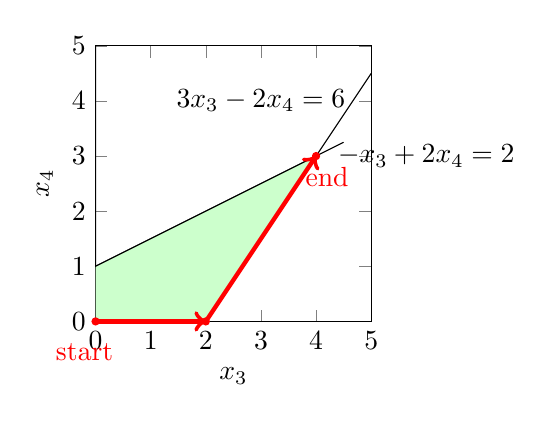
\begin{tikzpicture}[x=0.7cm,y=0.7cm]
%\pgfplotsset{my style/.append style={ axis x line=middle, axis y line=middle, axis equal }}
    \begin{axis}[anchor=origin,         xlabel=$x_3$,
        ylabel=$x_4$,
        xtick={ 0,..., 5},
        ytick={ 0,..., 5},
        xmin=0,
        xmax=5,
        ymin=0,
        ymax=5,
         x=0.7cm, y=0.7cm,
        ];
              \addplot[domain=0:4.5]{0.5*x+1};
              \addplot[domain=2:5]{1.5*x-3};
%              \addplot[domain=-1:3,-,red]{-x+1};


      \end{axis};
                    \node at (6,3) {$-x_3+2x_4 = 2$};
              \node at (3,4) {$3x_3-2x_4 = 6$};
%              \node[red] at (4,0) {$x_3+x_4=1$};
	\draw[fill=green!20] (0, 0) -- ( 2, 0) -- (4,3) -- (0,1) -- (0,05);
	\node[circle, minimum size=3pt,inner sep=0pt, fill=red] at (0,0) {};
		\node[circle, minimum size=3pt,inner sep=0pt, fill=red] at (2,0) {};
			\node[circle, minimum size=3pt,inner sep=0pt, fill=red] at (4,3) {};
			\node[below, red, ultra thick] at (-0.2,-0.2) {start};
			\node[below, red, ultra thick] at (4.2,3) {end};
			\draw[->, red, ultra thick] (0,0) -- (2,0);
			\draw[->, red, ultra thick] (2,0) -- (4,3);
\end{tikzpicture}


{\sc Improvement}()
\begin{algorithmic}[1]
\STATE $\mathbf{x=x_0}$;  \textcolor{red}{//starting from a vertex;}
\WHILE{ \texttt{TRUE} }
\STATE $\mathbf{x}=${\sc Improve}$(\mathbf{x})$; \textcolor{red}{//move to another vertex via an edge;}
\IF { {\sc stopping}$(\mathbf{x})$  }
\STATE break;  \textcolor{red}{ //stop when $\mathbf{x}$ is optimal}
\ENDIF
\ENDWHILE
\RETURN $\mathbf{x}$;
\end{algorithmic}

%\begin{figure}
%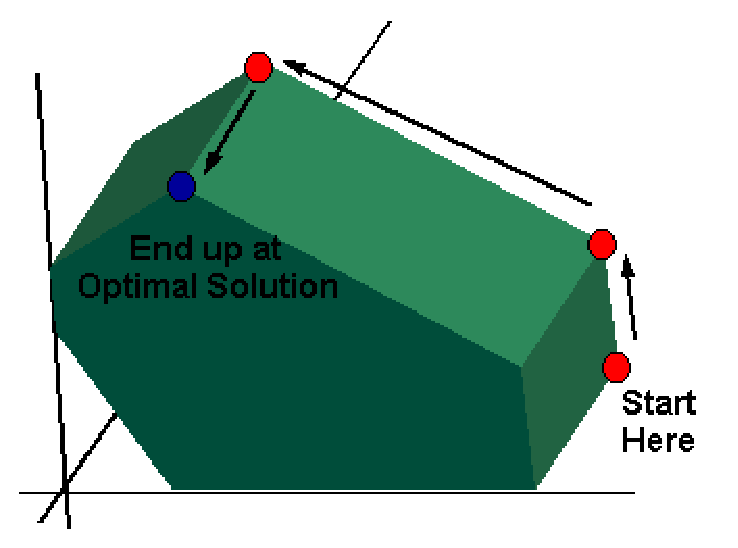
\includegraphics[width=1.7in]{L8-simplex.eps}
%\end{figure}

第一步:找到一个初始可行解,如$(0,0)$;
第二步:找到一个结果比$(0,0)$改进一点的点,比如$(2,0)$;发现还可以在改进,于是接着再改进一点,找到$ (4,3)$;
第三步:发现没有办法再改进了,则返回。

\textbf{注意:}琢磨清楚三句话,初始点怎么找,怎样改进,结束条件是什么。线性规划的单纯型算法、牛顿法之类的算法全都是这三句话。

我们来看一下,单纯型算法回答了哪些问题呢?

\begin{enumerate}
		\item 为什么我们只用考虑多胞形的顶点就够了呢?
		\item 怎样选择初始点?
		\item 怎样改进?
		\item 什么时候结束?
	\end{enumerate}


我们来一一回答。

\subsection{为什么我们只用考虑多胞形的顶点就够了呢?}

\begin{center}
 \includegraphics[width=2in] {L8-LP-GE3.png}
\end{center}

直观地看,我们发现最优解一定在顶点上,不需要考虑内部点,问题得到了极大的简化。

%1527行

%\begin{Theorem}
\textbf{定理:}
There exists a vertex in $\mathbf{P}$ that takes the optimal value.
%\end{Theorem}

%\begin{Proof}
\textbf{证明:}
\begin{itemize}
\begin{footnotesize}
 \item Since $\mathbf{P}$ is a bounded close set, $\mathbf{c^Tx}$ reaches its optimum in $\mathbf{P}$.
 \item Denote the optimal solution as $\mathbf{x}^{(0)}$. We will show there is a vertex at least as good as $\mathbf{x^{(0)} }$. Why?
\begin{itemize}
\begin{footnotesize}
 \item $\mathbf{x^{(0)} }$ can be represented as the convex combination of vertices of $\mathbf{P}$, i.e.  $\mathbf{x^{(0)} } = \lambda_1 \mathbf{x^{(1)} } + \lambda_2 \mathbf{x^{(2)} } + ... + \lambda_{k} \mathbf{x^{(k)} }$, where $\lambda_i \geq 0, \lambda_1 + ... + \lambda_{k} = 1 $.  (See Appendix for details.)
 \item Thus $\mathbf{c^Tx}^{(0)} = \lambda_1 \mathbf{ c^Tx}^{(1)} + \lambda_2 \mathbf{ c^Tx}^{(2)} + ... + \lambda_{k} \mathbf{ c^Tx}^{(k)}$
 \item Let $x^{(i)}$ be the vertex with the minimal objective value $\mathbf{ c^T x}^{(i)}$;
 \item $\mathbf{c^Tx}^{(0)} = \lambda_1 \mathbf{ c^T x}^{(1)} + \lambda_2 \mathbf{ c^T x}^{(2)} + ... + \lambda_{k} \mathbf{ c^T x}^{(k)} \geq \mathbf{ c^T x}^{(i)} $.
% \end{footnotesize}
\end{footnotesize}
\end{itemize}
 \item Thus,  vertex $\mathbf{x}^{(i)}$ is also an optimal solution  since $\mathbf{ c^T x}^{(i)} \leq \mathbf{c^Tx}^{(0)}$ \end{footnotesize}
\end{itemize}
%\end{Proof}

\begin{center}
  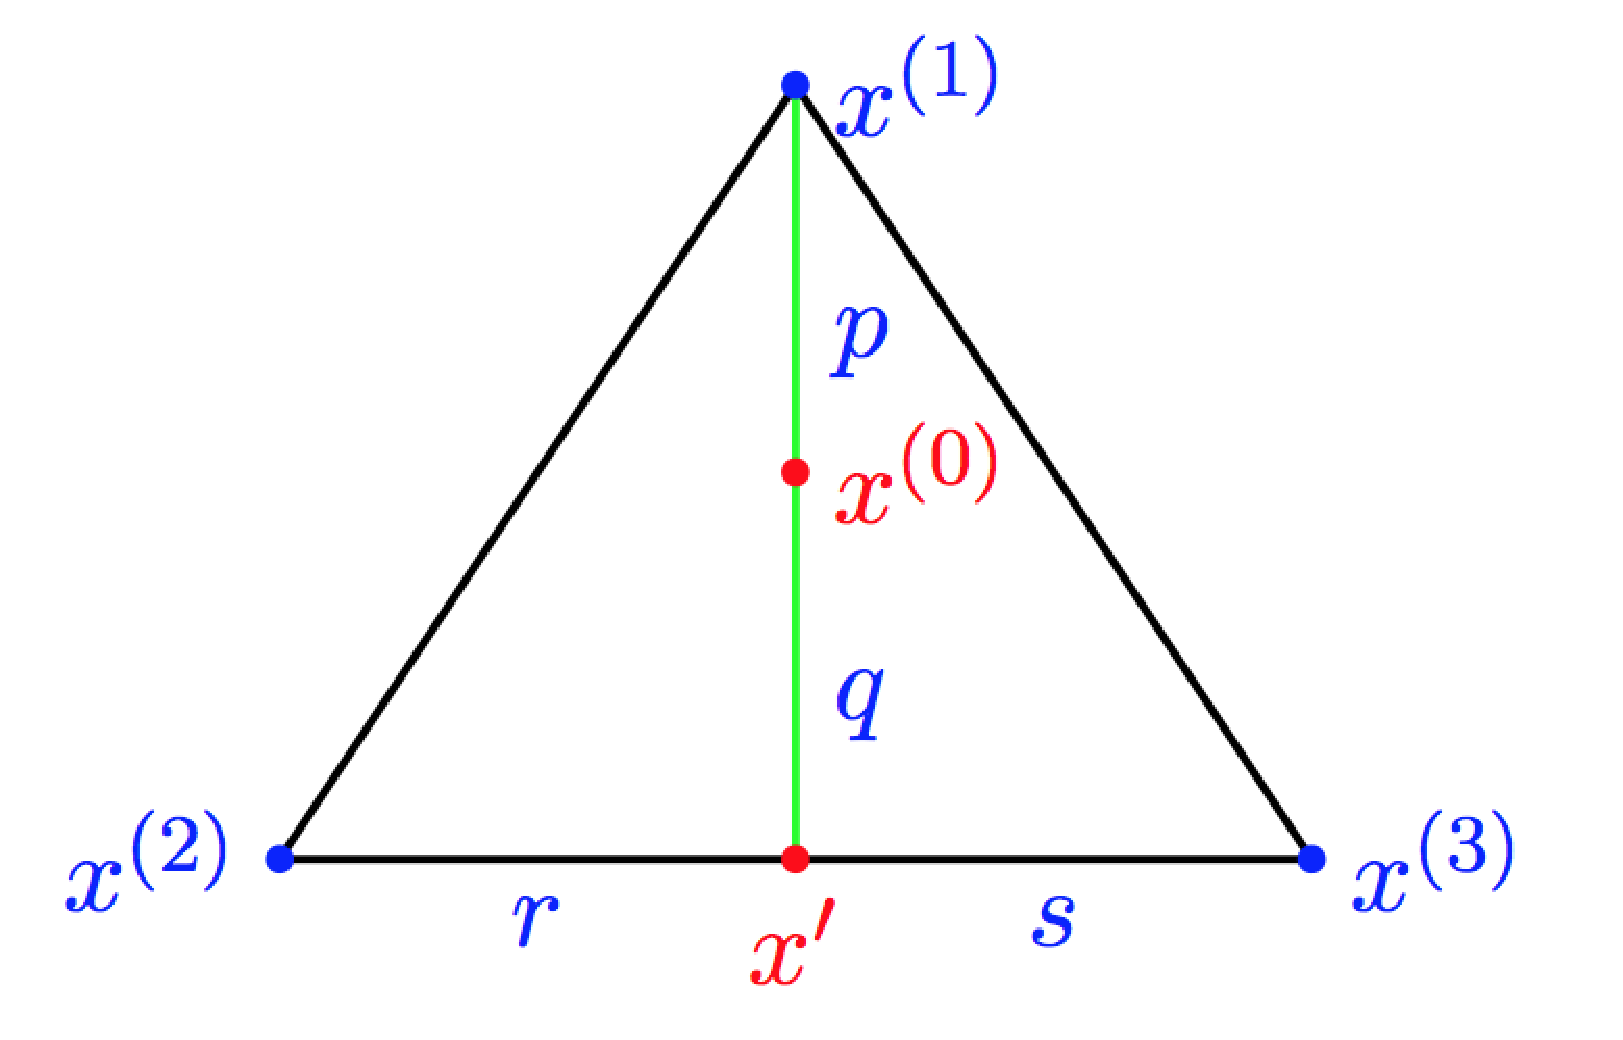
\includegraphics[width=1.4in] {L8-x1x2x3.eps}
\end{center}

\begin{itemize}
\item Suppose $\mathbf{x}^{(0)}$ is an optimal solution.
 \item Connecting $\mathbf{x}^{(0)}$ and $\mathbf{x}^{(1)}$ with a line. Suppose the line intersects line segment $(\mathbf{x}^{(2)}, \mathbf{x}^{(3)} )$ at point $\mathbf{x}'$.
 \item We have $\mathbf{x}^{(0)} = \lambda_1\mathbf{x}^{(1)} + (1-\lambda_1) \mathbf{x}'$, where $\lambda_1 = \frac{p}{p+q}$.
 \item We also have $\mathbf{x}'= \lambda_2 \mathbf{x}^{(2)} + (1-\lambda_2) \mathbf{x}^{(3)} $, where $\lambda_2 = \frac{r}{r+s}$.
 \item Thus, we have $\mathbf{x}^{(0)} = \lambda_1 \mathbf{x}^{(1)} + (1-\lambda_1)\lambda_2 \mathbf{x}^{(2)} + (1-\lambda_1)(1-\lambda_2) \mathbf{x}^{(3)}$.
 \item Suppose $\mathbf{ c^T x^{(1)} }$ is the minimum of $\mathbf{c^Tx^{(1)}, c^Tx^{(2)}, c^Tx^{(3)} }$.
 \item Notice that $\lambda_1  +  (1-\lambda_1)\lambda_2 + (1-\lambda_1)(1-\lambda_2) = 1$.
  \item We have: $\mathbf{ c^T x^{(1)}} \leq \mathbf{ c^T x^{(0)}}$. Thus, a vertex $\mathbf{x}^{(1)}$ is found not worse than $\mathbf{x}^{(0)}$.
\end{itemize}

\subsection{怎样选择初始点?}
\begin{center}
   \includegraphics[width=1.1in] {L8-LPexample3D.eps}
\end{center}

考虑一个三维的多胞体,我们已经知道,对于我们所要求解的问题,只用考虑顶点就够了,内部点不用考虑。

我们人通过看图很容易得到这些顶点,那么,怎样写程序找到多胞体的顶点?

\textbf{定理:}
A vertex of $\mathbf{P}$ corresponds to a basis of matrix $\mathbf{A}$.

一个多边形的顶点就对应着一个矩阵的基,这下就好做了,只要给一个矩阵求基就行了。

\textbf{例子:}

\begin{scriptsize}
\[
\begin{array}{rrrrrrrrrrrrl}
 \min & - x_1     &-&  14 x_2    &-& 6 x_3 \\
 s.t. &   x_1     &+&     x_2    &+& x_3 & \leq & 4   \\
      &   x_1     & &            & &     & \leq & 2   \\
      &           & &            & &  x_3& \leq & 3   \\
      &           & &   3x_2     &+&  x_3& \leq & 6   \\
      &   x_1     &,&   x_2      &,&  x_3& \geq & 0   \\
\end{array} \nonumber
\]
\end{scriptsize}


\textbf{证明:}

\textbf{Part 1: Vertex $\Rightarrow$ basic feasible solution}
\begin{itemize}
\item
We will first show that \textcolor{red}{\bf any vertex} of the polytope corresponds to a basis of the matrix $\mathbf{A}$.
\item
An example (slack form):
\begin{scriptsize}
\[
\begin{array}{rrrrrrrrrrrrrrrrl}
 \min & - x_1     &-&  14 x_2    &-& 6 x_3 & &  & & & & & &\\
 s.t. &   x_1     &+&     x_2    &+& x_3  &+ & x_4 & & & & & &   			& = & 4   \\
      &   x_1     & &            & &               & &  &+ & x_5& & & & 			& = & 2   \\
      &           & &            & &  x_3	  & &  & & &+ & x_6& &			& = & 3   \\
      &           & &   3x_2     &+&  x_3	  & &  & & & & & +&x_7			& = & 6   \\
      &   x_1     &,&   x_2      &,&  x_3    &, & x_4 &, &x_5 &, & x_6& ,&	x_7	        & \geq & 0   \\
\end{array} \nonumber
\]
\end{scriptsize}

\begin{center}
  \includegraphics[width=1.1in] {L8-LPexample3D.eps}
\end{center}
\end{itemize}

\textbf{矩阵描述:}
%\begin{figure}%
   \begin{center}%
     \begin{minipage}{0.3\textwidth}%
      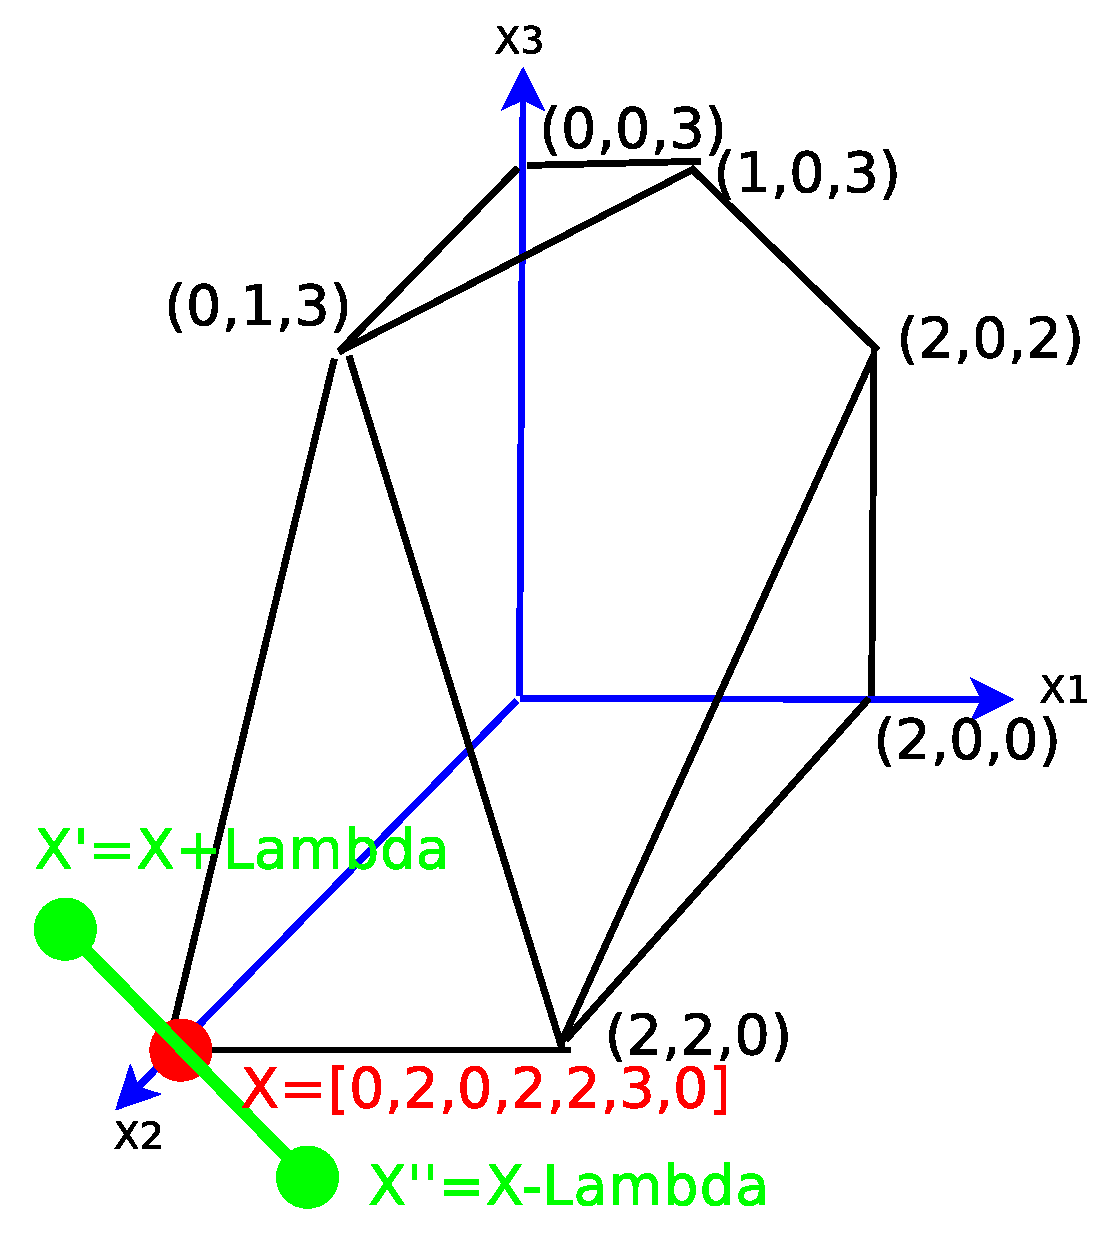
\includegraphics[width=1.0\textwidth]{L8-LPexample3Dvertex.eps}%
     \end{minipage}%
     \quad
     \begin{minipage}{0.36\textwidth}
      \includegraphics[width=1.0\textwidth]{L8-LPexample3Dvertexmatrix.png}%
     \end{minipage}%
   \end{center}
 %\end{figure}

\textbf{补充:}关于矩阵的描述,推荐大家看一本书,\emph{ Linear Algebra and Its Applications (David C. Lay) }。

 \begin{itemize}
 \item Take the vertex $(x_1, x_2, x_3) = (0,2,0)$ as an example. The corresponding full solution is $(x_1,x_2,x_3,x_4,x_5,x_6,x_7)= ( 0, 2, 0, 2, 2, 3, 0)$.
  \item We will show that the column vectors corresponding to \textcolor{blue}{\bf non-zero $x_i$}, i.e. $\mathbf{ \textcolor{blue}{ \{a_2, a_4, a_5, a_6 \}}}$, are linearly independent.
  \item Suppose $\exists (\lambda_2, \lambda_4, \lambda_5,\lambda_6) \neq 0$ such that $\lambda_{2}\mathbf{a_{2}} + \lambda_{4}\mathbf{a_{4}} + \lambda_{5}\mathbf{a_{5}}+ \lambda_{6}\mathbf{a_{6}}  = 0$, i.e. $\mathbf{A\lambda=0}$, where $\mathbf{\lambda} = [0, \lambda_2, 0, \lambda_4, \lambda_5,\lambda_6, 0]$.
\item Then we can construct \textcolor{green}{\bf two other points: $\mathbf{x'=x+\theta \lambda}$ and $\mathbf{x''=x-\theta \lambda}$. }
\item It is easy to deduce  that both $\mathbf{x'}$ and $\mathbf{x''}$ lie inside $P$ since:
\begin{itemize}
\begin{scriptsize}
\item $\mathbf{A x' = Ax + 0 = b}$ and   $\mathbf{A x'' = Ax - 0 = b}$
\item In addition, we can guarantee $\mathbf{x' \geq 0}$ and  $\mathbf{x'' \geq 0}$ via setting $\theta$ to be sufficiently small since $\mathbf{x \geq 0}$, and $\lambda_1=\lambda_3=\lambda7=0$.
\end{scriptsize}
\end{itemize}
 \item Contradiction: it is impossible for a vertex to be  center of two inner points of $\mathbf{P}$.
 \end{itemize}

 现在我们已经知道顶点可以表示成基,我们来把过去的东西用矩阵的语言表示。对于任何一个顶点,都对应一个基$B$,我们把非基的列都叫做$N$。于是有,
\begin{itemize}
\item For a vertex $\mathbf{x}$ of the polytope, a basis $\mathbf{B}$ can be derived via extracting the column vectors corresponding to non-zero $x_i$. The non-basis column vectors are denoted as $\mathbf{N}$.
\item Then  the original LP  can be represented as:

%\begin{center}
%  \includegraphics[width=2.5in] {L8-simplextable.png}
%\end{center}

 \item Here, $\mathbf{x}$  is decomposed as $\mathbf{x=\left[\begin{array}{c}\mathbf{x_B}\\\mathbf{x_N}\end{array}\right]}$. Then  we have $\mathbf{x_N=0}$, and $\mathbf{x_B=B^{-1}b}$ (Reason: $\mathbf{Ax=b}$, i.e. $\mathbf{B x_B + N x_N = b}$ )
 \item The corresponding objective value is $\mathbf{c^T x = c_B^T x_B + c_N^T x_N = c_B^T B^{-1} b }$.
 \end{itemize}


\textbf{一个例子:}
\begin{itemize}
 \item For a vertex $\mathbf{x}= \ \left[ \begin{array}{ccccccc}
               0 &\textcolor{blue}{2} &0 &\textcolor{blue}{2} &\textcolor{blue}{2} &\textcolor{blue}{3} &0
               \end{array}
               \right]^T$, the columns corresponding to non-zero $x_i$ are extracted to form a basis
$ \mathbf{B} = \left[
			\begin{array}{cccc}
		 \textcolor{blue}{1} &  \textcolor{blue}{1} & \textcolor{blue}{0} & \textcolor{blue}{0}  \\
		 \textcolor{blue}{0} &  \textcolor{blue}{0} & \textcolor{blue}{1} & \textcolor{blue}{0}  \\
		 \textcolor{blue}{0} &  \textcolor{blue}{0} & \textcolor{blue}{0} & \textcolor{blue}{1}  \\
		 \textcolor{blue}{3} &  \textcolor{blue}{0} & \textcolor{blue}{0} & \textcolor{blue}{0}
			\end{array}
			\right]$.
\item Let's decompose $\mathbf{x}= \ \left[ \begin{array}{ccccccc}
               0 &\textcolor{blue}{2} &0 &\textcolor{blue}{2} &\textcolor{blue}{2} &\textcolor{blue}{3} &0
               \end{array}
               \right]^T
$ accordingly into  $ \mathbf{x_B}=[\textcolor{blue}{2\ 2\ 2\ 3}]^T$\text{ and }  $\mathbf{x_N}=[0\ 0\ 0]^T$.
\item It is easy to verify that $\mathbf{x_B = B^{-1}b}$. In this example, $\mathbf{b} = \left[ \begin{array}{c}
						4\\
						2\\
						3\\
						6
					 	\end{array} \right]$.

 \end{itemize}

\textbf{ Part 2: Basic feasible  solution  $\Rightarrow$ vertex}
\begin{itemize}
\item Given a  basis $\mathbf{B}$ of matrix $\mathbf{A}$,  we call $\mathbf{x=\left[\begin{array}{c}\mathbf{B^{-1}b}\\\mathbf{0}\end{array}\right]}$ a  \textcolor{red}{\bf basic solution respect to $\mathbf{B}$}.
 \item If we further have $\mathbf{x_B = B^{-1}b \geq 0 }$, $\mathbf{x}$ is called  a \textcolor{red}{\bf basic feasible solution respect to $\mathbf{B}$}.
 \item We will show that a \textcolor{red}{\bf basic feasible solution $\mathbf{x}$ respect to $\mathbf{B}$} is a vertex of the polytope $\mathbf{P}$.
  \end{itemize}

\textbf{证明:}
\begin{itemize}
\begin{small}
 \item It suffices to show that $\mathbf{x}$ cannot be represented as a convex combination of any two points in $\mathbf{P}$.
\item By contradiction, suppose there are two different points $\mathbf{x^{(1)}}$ and $\mathbf{x^{(2)}}$ in $\mathbf{P}$ such that $\mathbf{x} = \lambda_1 \mathbf{x^{(1)}} + \lambda_2 \mathbf{x^{(2)}}$, where $0 < \lambda_1, \lambda_2 < 1$.
\item Note that $\lambda_1 \mathbf{x^{(1)}_N} + \lambda_2 \mathbf{x^{(2)}_N} = \mathbf{x_N} = 0$.
\item So $\mathbf{x^{(1)}_N} = \mathbf{x^{(2)}_N} = 0$.
\item We have  $\mathbf{x^{(1)}_B} = \mathbf{x^{(2)}_B} = \mathbf{B^{-1}b} = \mathbf{x_B}$ (by $\mathbf{Ax^{(1)}=0}$ and  $\mathbf{Ax^{(2)}=0}$). A contradiction.
\end{small}
 \end{itemize}

 \textbf{一个例子:}
 \begin{itemize}
\item
For matrix $\mathbf{A}=\left[
		\begin{array}{ccccccc}
		1 & \textcolor{blue}{1} & 1 & \textcolor{blue}{1} & \textcolor{blue}{0} & \textcolor{blue}{0} & 0 \\
		1 & \textcolor{blue}{0} & 0 & \textcolor{blue}{0} & \textcolor{blue}{1} & \textcolor{blue}{0} & 0 \\
		0 & \textcolor{blue}{0} & 1 & \textcolor{blue}{0} & \textcolor{blue}{0} & \textcolor{blue}{1} & 0 \\
		0 & \textcolor{blue}{3} & 1 & \textcolor{blue}{0} & \textcolor{blue}{0} & \textcolor{blue}{0} & 1
		\end{array}
		\right],
		 \text{ and } \mathbf{b} = \left[ \begin{array}{c}
						4\\
						2\\
						3\\
						6
					 	\end{array} \right]
$, we first calculate a basis of $\mathbf{A}$ as
 $\mathbf{B} = \left[
			\begin{array}{cccc}
		 \textcolor{blue}{1} &  \textcolor{blue}{1} & \textcolor{blue}{0} & \textcolor{blue}{0}  \\
		 \textcolor{blue}{0} &  \textcolor{blue}{0} & \textcolor{blue}{1} & \textcolor{blue}{0}  \\
		 \textcolor{blue}{0} &  \textcolor{blue}{0} & \textcolor{blue}{0} & \textcolor{blue}{1}  \\
		 \textcolor{blue}{3} &  \textcolor{blue}{0} & \textcolor{blue}{0} & \textcolor{blue}{0}
			\end{array}
			\right]$.
%
%			$  \mathbf{N}= \left[
%			\begin{array}{ccc}
%			1 & 1 & 0 \\
%			1 & 0 & 0 \\
%			0 & 1 & 0 \\
%			0 & 1 & 1
%			\end{array}
%			\right],
%			$\\
%\ \\
\item
The  \textcolor{red}{\bf basic feasible solution $\mathbf{x}$ respect to $\mathbf{B}$} is   $\mathbf{x=\left[\begin{array}{c}\mathbf{B^{-1}b}\\\mathbf{0}\end{array}\right]} = \ \left[ \begin{array}{ccccccc}
               0 &\textcolor{blue}{2} &0 &\textcolor{blue}{2} &\textcolor{blue}{2} &\textcolor{blue}{3} &0
               \end{array}
               \right]^T
$.
\item
It is easy to verify  that $(x_1, x_2, x_3) = (0, 2, 0)$ is a vertex of the polytope $\mathbf{P}$.
\end{itemize}




